% Options for packages loaded elsewhere
\PassOptionsToPackage{unicode}{hyperref}
\PassOptionsToPackage{hyphens}{url}
%
\documentclass[
  a4paper,
]{scrbook}

\usepackage{amsmath,amssymb}
\usepackage{iftex}
\ifPDFTeX
  \usepackage[T1]{fontenc}
  \usepackage[utf8]{inputenc}
  \usepackage{textcomp} % provide euro and other symbols
\else % if luatex or xetex
  \usepackage{unicode-math}
  \defaultfontfeatures{Scale=MatchLowercase}
  \defaultfontfeatures[\rmfamily]{Ligatures=TeX,Scale=1}
\fi
\usepackage{lmodern}
\ifPDFTeX\else  
    % xetex/luatex font selection
  \setmainfont[]{Latin Modern Roman}
  \setsansfont[]{Latin Modern Roman}
\fi
% Use upquote if available, for straight quotes in verbatim environments
\IfFileExists{upquote.sty}{\usepackage{upquote}}{}
\IfFileExists{microtype.sty}{% use microtype if available
  \usepackage[]{microtype}
  \UseMicrotypeSet[protrusion]{basicmath} % disable protrusion for tt fonts
}{}
\makeatletter
\@ifundefined{KOMAClassName}{% if non-KOMA class
  \IfFileExists{parskip.sty}{%
    \usepackage{parskip}
  }{% else
    \setlength{\parindent}{0pt}
    \setlength{\parskip}{6pt plus 2pt minus 1pt}}
}{% if KOMA class
  \KOMAoptions{parskip=half}}
\makeatother
\usepackage{xcolor}
\setlength{\emergencystretch}{3em} % prevent overfull lines
\setcounter{secnumdepth}{5}
% Make \paragraph and \subparagraph free-standing
\ifx\paragraph\undefined\else
  \let\oldparagraph\paragraph
  \renewcommand{\paragraph}[1]{\oldparagraph{#1}\mbox{}}
\fi
\ifx\subparagraph\undefined\else
  \let\oldsubparagraph\subparagraph
  \renewcommand{\subparagraph}[1]{\oldsubparagraph{#1}\mbox{}}
\fi


\providecommand{\tightlist}{%
  \setlength{\itemsep}{0pt}\setlength{\parskip}{0pt}}\usepackage{longtable,booktabs,array}
\usepackage{calc} % for calculating minipage widths
% Correct order of tables after \paragraph or \subparagraph
\usepackage{etoolbox}
\makeatletter
\patchcmd\longtable{\par}{\if@noskipsec\mbox{}\fi\par}{}{}
\makeatother
% Allow footnotes in longtable head/foot
\IfFileExists{footnotehyper.sty}{\usepackage{footnotehyper}}{\usepackage{footnote}}
\makesavenoteenv{longtable}
\usepackage{graphicx}
\makeatletter
\def\maxwidth{\ifdim\Gin@nat@width>\linewidth\linewidth\else\Gin@nat@width\fi}
\def\maxheight{\ifdim\Gin@nat@height>\textheight\textheight\else\Gin@nat@height\fi}
\makeatother
% Scale images if necessary, so that they will not overflow the page
% margins by default, and it is still possible to overwrite the defaults
% using explicit options in \includegraphics[width, height, ...]{}
\setkeys{Gin}{width=\maxwidth,height=\maxheight,keepaspectratio}
% Set default figure placement to htbp
\makeatletter
\def\fps@figure{htbp}
\makeatother

\usepackage{booktabs}
\usepackage{longtable}
\usepackage{array}
\usepackage{multirow}
\usepackage{wrapfig}
\usepackage{float}
\usepackage{colortbl}
\usepackage{pdflscape}
\usepackage{tabu}
\usepackage{threeparttable}
\usepackage{threeparttablex}
\usepackage[normalem]{ulem}
\usepackage{makecell}
\usepackage{xcolor}
\usepackage{titling}
\setlength{\droptitle}{-2cm}
\preauthor{
  \begin{center}
  \Large
  \vspace{10mm}
  by

  \vspace{20mm}
}
\postauthor{
  \end{center}
  \vfill
}

\predate{
  \begin{center}
  A thesis 
  submitted in fulfilment of the \\
  requirements of the degree of \\
  Doctor of Philosophy in Physics\\               % Degree
  School of Physical and Chemical Sciences\\          % Department
  Te Herenga Waka - Victoria University of Wellington\\                       % University 
  \vspace{5mm}
}
\postdate{
  \\
  
\includegraphics[width=3in,height=1.5in]{figures/VUW-logo.png}\\
  \end{center}
  }
\makeatletter
\makeatother
\makeatletter
\@ifpackageloaded{bookmark}{}{\usepackage{bookmark}}
\makeatother
\makeatletter
\@ifpackageloaded{caption}{}{\usepackage{caption}}
\AtBeginDocument{%
\ifdefined\contentsname
  \renewcommand*\contentsname{Table of contents}
\else
  \newcommand\contentsname{Table of contents}
\fi
\ifdefined\listfigurename
  \renewcommand*\listfigurename{List of Figures}
\else
  \newcommand\listfigurename{List of Figures}
\fi
\ifdefined\listtablename
  \renewcommand*\listtablename{List of Tables}
\else
  \newcommand\listtablename{List of Tables}
\fi
\ifdefined\figurename
  \renewcommand*\figurename{Figure}
\else
  \newcommand\figurename{Figure}
\fi
\ifdefined\tablename
  \renewcommand*\tablename{Table}
\else
  \newcommand\tablename{Table}
\fi
}
\@ifpackageloaded{float}{}{\usepackage{float}}
\floatstyle{ruled}
\@ifundefined{c@chapter}{\newfloat{codelisting}{h}{lop}}{\newfloat{codelisting}{h}{lop}[chapter]}
\floatname{codelisting}{Listing}
\newcommand*\listoflistings{\listof{codelisting}{List of Listings}}
\makeatother
\makeatletter
\@ifpackageloaded{caption}{}{\usepackage{caption}}
\@ifpackageloaded{subcaption}{}{\usepackage{subcaption}}
\makeatother
\makeatletter
\@ifpackageloaded{tcolorbox}{}{\usepackage[skins,breakable]{tcolorbox}}
\makeatother
\makeatletter
\@ifundefined{shadecolor}{\definecolor{shadecolor}{rgb}{.97, .97, .97}}
\makeatother
\makeatletter
\makeatother
\makeatletter
\makeatother
\ifLuaTeX
  \usepackage{selnolig}  % disable illegal ligatures
\fi
\usepackage[citestyle = ieee,urldate = iso8601]{biblatex}
\addbibresource{references.bib}
\IfFileExists{bookmark.sty}{\usepackage{bookmark}}{\usepackage{hyperref}}
\IfFileExists{xurl.sty}{\usepackage{xurl}}{} % add URL line breaks if available
\urlstyle{same} % disable monospaced font for URLs
\hypersetup{
  pdftitle={Volatile Organic Compound Detection Using Insect Odorant-Receptor Functionalised Field-Effect Transistors},
  pdfauthor={Eddyn Oswald Perkins Treacher},
  hidelinks,
  pdfcreator={LaTeX via pandoc}}

\title{Volatile Organic Compound Detection Using Insect Odorant-Receptor
Functionalised Field-Effect Transistors}
\author{Eddyn Oswald Perkins Treacher}
\date{Mar 2024}

\begin{document}
\frontmatter
\maketitle
\ifdefined\Shaded\renewenvironment{Shaded}{\begin{tcolorbox}[frame hidden, enhanced, breakable, boxrule=0pt, interior hidden, borderline west={3pt}{0pt}{shadecolor}, sharp corners]}{\end{tcolorbox}}\fi

\renewcommand*\contentsname{Table of contents}
{
\setcounter{tocdepth}{2}
\tableofcontents
}
\mainmatter
\bookmarksetup{startatroot}

\hypertarget{acknowledgements}{%
\chapter*{Acknowledgements}\label{acknowledgements}}
\addcontentsline{toc}{chapter}{Acknowledgements}

\markboth{Acknowledgements}{Acknowledgements}

\begin{verbatim}
69450
\end{verbatim}

Rifat, Alex - vapour sensor Erica Cassie - FET sensing setup Rob Keyzers
and Jennie Ramirez-Garcia - NMR spectra Patricia Hunt - Computational
chemistry

\bookmarksetup{startatroot}

\hypertarget{sec-vapour-sensing-biosensors}{%
\chapter{Vapour Sensing System for Transistor
Biosensing}\label{sec-vapour-sensing-biosensors}}

\hypertarget{general-remarks}{%
\section{General Remarks}\label{general-remarks}}

Through the adaptation of an existing setup, a custom vapour delivery
system was developed to measure the response of field-effect biosensors
to vapour. To achieve this goal, the new system needed to meet three
requirements:

\begin{itemize}
\item
  The ability to automatically deliver a vapour to an enclosed
  environment in a controlled manner.
\item
  The ability to collect measurements from a sensor device within that
  environment.
\item
  The ability to collect data from off-the-shelf reference sensors
  monitoring the same environment, for comparison with data collected by
  the novel biosensor.
\end{itemize}

The previously existing system had a limited ability to meet the first
two requirements, but was not able to take reference measurements of
vapour flow. To implement new elements that would enable the system to
fulfill all three requirements, a two-step development approach was
taken across the course of the thesis. The changes made with each step
of the redesign are outlined in Section~\ref{sec-vapour-system-design}.

Three mass flow controllers (MFC) were used to precisely control and
monitor the flow of nitrogen into the system in units of standard cubic
centimeters per minute (sccm). The manner in which these controllers
were configured in the system is discussed in
Section~\ref{sec-delivery-system}. The reference sensors chosen were a
photoionisation detector (Ametek Mocon) and relative humidity and
temperature indicator (Telaire). The photoionisation detector is able to
monitor a wide range of volatile organic compounds, but cannot monitor
compounds with an ionisation energy exceeding 10.6 eV. This includes
nitrogen, oxygen, carbon dioxide, argon and water
\autocite{PIDmanual,Ionscience}. Therefore, the photoionisation detector
(PID) should not respond to either ambient air or standard nitrogen flow
through the detector. As we would also like to monitor the presence of
water vapour in the system, we use the relative humidity indicator
(RHI). The operation of these reference sensors is discussed further in
Section~\ref{sec-reference-sensors}.

\hypertarget{technical-notes}{%
\section{Technical Notes}\label{technical-notes}}

\hypertarget{sec-delivery-system}{%
\subsection{Delivery System}\label{sec-delivery-system}}

\begin{figure}

{\centering \includegraphics[width=0.7\textwidth,height=\textheight]{figures/ch5/vapour_system_layout_2.png}

}

\caption{\label{fig-mass-flow-controller-layout}Image of the three mass
flow controllers (MFCs) of the Te Herenga Waka - Victoria University of
Wellington cleanroom vapour delivery system, each with a regulator to
set the pressure at the MFC inlet. (1) is the 20 sccm full-scale flow
MFC, (2) is the 200 sccm full-scale flow MFC, and (3) is the 500 sccm
full-scale flow MFC.}

\end{figure}

\begin{figure}

{\centering \includegraphics[width=0.7\textwidth,height=\textheight]{figures/ch5/analyte_bottle.png}

}

\caption{\label{fig-analyte-bottle}Image of the analyte bottle, used to
hold a volatile compound which provides vapour to the carrier line,
either through bubbling or headspace sampling.}

\end{figure}

Three mass flow controller and their associated regulators sit in an
covered enclosure, seen from the front in
Figure~\ref{fig-mass-flow-controller-layout}. These are used to control
the nitrogen flow rate through two different lines towards the chamber,
the carrier line and dilution line. The lines merge at a mixing point
about a metre before the device chamber, which contains the device being
analysed. Each line consist of a mix of stainless steel and flexible PVC
tubing, with various Swagelok fittings and valves. These valves include
check valves, to ensure there is no backflow of vapour within the
system. The carrier line connects flow to a 10 mL Schott bottle (Duran)
containing analyte, shown in Figure~\ref{fig-analyte-bottle}. The vapour
from the volatile analyte is then carried by nitrogen flow through the
carrier line. A three-way valve determines whether the analyte vapour is
then carried towards the mixing point or sent into the fumehood via the
exhaust. The dilution line separately delivers flow to the mixing point,
modifying the flow pushing the analyte vapour towards the chamber.

The setup is designed so that only one mass flow controller is directed
through a single line at a time. The mass flow controller with a
full-scale flow of 500 sccm (standard cubic centimeters per minute) can
only be directed through the dilution line, and the mass flow controller
with a full-scale flow of 20 sccm can only be directed through the
carrier line. The mass flow controller with a full-scale flow of 200
sccm can be directed through the dilution line or carrier line. The
electronic integration and programming of the mass flow controllers is
described in Section~\ref{sec-control-system}.

\hypertarget{sec-reference-sensors}{%
\subsection{Reference Sensors}\label{sec-reference-sensors}}

\begin{figure}

{\centering \includegraphics[width=0.7\textwidth,height=\textheight]{figures/ch5/vapour_system_layout_1.png}

}

\caption{\label{fig-reference-sensor-layout}Image of the device chamber,
reference sensors and other related components. The components are
labelled as follows: (1) Device chamber, (2) Photoionisation detector
(PID), (3) Flowmeter from chamber to PID, (4) Micropump from chamber to
PID, (5) Relative humidity and temperature monitor.}

\end{figure}

Two reference sensors were added to the vapour delivery setup to compare
the response to vapour by the fabricated sensor device with some
reference signal. These reference sensors are a photoionisation detector
(Ametek Mocon) and a relative humidity and temperature indicator
(Telaire). The layout of these reference sensors (and their associated
peripherals) relative to the device chamber is shown in
Figure~\ref{fig-reference-sensor-layout}. These components are on a
raised platform directly above the mass flow controller enclosure.
Vapour flowing through the device chamber passes into a cylindrical
manifold with three outlets. One outlet is the system exhaust, one flows
into relative humidity indicator chamber, and one flows into the
photoionisation detector. A dial-controlled micro diaphragm pump is used
to set the flow rate from the manifold into the photoionisation
detector, with a flowmeter used to monitor this flow rate.

The electronic integration and programming of the relative humidity and
temperature indicator is described in Section~\ref{sec-control-system}.
The photoionisation detector was connected to a laptop directly via USB,
then controlled and monitored using the supplier-provided VOC-TRAQ II
software package.

\hypertarget{relative-humidity-and-temperature-indicator}{%
\subsubsection*{Relative Humidity and Temperature
Indicator}\label{relative-humidity-and-temperature-indicator}}
\addcontentsline{toc}{subsubsection}{Relative Humidity and Temperature
Indicator}

The relative humidity and temperature indicator used here is a
capacitive humidity sensor \autocite{Telairesensor}. It consists of a
capacitor with a hygroscopic polymer as the capacitor dielectric. As
room temperature water has a much larger dielectric constant than the
polymer dielectric, absorption of water by the polymer leads to
increased sensor capacitance \autocite{capacitivesensor}. The sensor
capacitance, corresponding to the amount of moisture absorbed by the
polymer and therefore the relative humidity, is then translated by the
sensor into a calibrated electronic output. This output is then
processed using the hardware and software described in
Section~\ref{sec-control-system} to give a value for the relative
humidity. The sensor has a quoted relative humidity (RH) accuracy of
\(\pm 2.0\)\% when RH is below 80\%, and has a quoted temperature
accuracy of \(0.5^\circ\)C \autocite{Telairesensor}.

The absolute humidity (AH), the mass of water vapour within a set
volume, can be calculated in gm\(^{-3}\) using
Equation~\ref{eq-absolute-humidity}, where \(C = 2.16679\) gKJ\(^{-1}\),
\(P_W\) is the water vapour pressure (in Pa) and T is the temperature
(in K) \autocite{humidityformula}.

\begin{equation}\protect\hypertarget{eq-absolute-humidity}{}{
AH = C\frac{P_W}{T}
}\label{eq-absolute-humidity}\end{equation}

For temperatures between -20 \(^\circ\)C and 50 \(^\circ\)C, water
vapour pressure \(P_W\) (in hPa) can be approximated using
Equation~\ref{eq-water-vapour-pressure}, where RH is relative humidity,
T is temperature in \(^\circ\)C, \(A = 6.116441\) hPa, \(m = 7.591386\)
and \(T_{n} = 240.7263 ^\circ\)C \autocite{humidityformula}.

\begin{equation}\protect\hypertarget{eq-water-vapour-pressure}{}{
P_W = RH \times A \times 10^{(mT/(T+T_{n}))}
}\label{eq-water-vapour-pressure}\end{equation}

\hypertarget{photoionisation-detector}{%
\subsubsection*{Photoionisation
Detector}\label{photoionisation-detector}}
\addcontentsline{toc}{subsubsection}{Photoionisation Detector}

A photoionisation detector (PID) can be used to continuously monitor
volatile organic compounds by measuring the extent to which vapour
molecules passing through the detector can be ionised. A small
percentage of vapour molecules flowing into the detector diffuse into a
sensor cavity. This cavity is bounded on each side by a pair of
electrodes. A lamp in the body of the detector radiates UV light through
a window into this cavity. The vapour molecules have their outer-most
electrons excited and removed when struck with these high-energy
photons. The ionised molecules then drift towards the sensor cathode,
while free electrons drift towards the sensor anode. This results in a
current proportional to the concentration of vapour molecules in the
chamber. The current can then be amplified for a signal readout. To be
detected, the ionisation energy of the molecules being monitored cannot
exceed the energy of the incident UV light. Therefore, molecules of
clean air will not be detected. Likewise, volatile organic compounds
with high ionisation energy \(-\) such as methane \(-\) will not be
recognised by the PID. Conversely, if the energy is required to ionise a
volatile of interest is relatively low, the PID will generally show a
relatively large response to that volatile
\autocite{Ionscience,PIDmanual}.

The photoionisation detector used in this work had a lamp energy of 10.6
eV, with a quoted response time of less than 2 seconds. Photoionisation
detectors are designed to sensitively detect within a particular
concentration range. PID sensors can become less sensitive after being
exposed to very high concentrations of volatile gas. They can also
become less sensitive if exposed to high levels of humidity or volatile
substances known to contaminate the PID window, which are not used in
this thesis. The typical sensitivity range of a PID can be stated in
terms of the sensor response to isobutylene gas, which is typically used
to calibrate PID sensors. The sensitivity of the the PID sensor used
here was 10 ppb \(-\) 200 ppm. Calibration with a reference gas ensures
the detector reads the true concentration of volatiles being detected,
multiplied by some previously-documented factor called a ``response
factor''. However, these response factors can vary based on the design
of the PID and various environmental factors
\autocite{Ionscience,PIDmanual}.

In this work, the PID was operated without end-user calibration. PID
measurements were used to confirm the evolution of vapour presence in
the chamber over time. It should be expected that sensor sensitivity
will exhibit span drift over days or weeks, depending on changes in the
local environment, and therefore measurements should not be treated as
absolute measurements that correspond to a true concentration reading.

The vapour of interest can be delivered to the PID either through
diffusion or by means of a low-power pump. A micro diaphragm pump
(Xavitech) was selected to pump the vapour from the chamber into the PID
detector. A pump with a low maximum flow rate was selected since the PID
requires a inlet flow of less than 300 sccm. As the pump is controlled
using a unlabelled dial, a flowmeter was used to independently measure
the flow rate through the micropump into the PID.

\hypertarget{sec-control-system}{%
\subsection{Control System}\label{sec-control-system}}

The vapour delivery system was controlled and monitored from a laptop
connected to a National Instruments USB-6009 multifunction data
acquisition input/ output module (DAQ). This USB-6009 DAQ connected to
the mass flow controllers and relative humidity and temperature
indicator (Telaire) via a custom-designed circuit board manufactured by
PCBway. The outputs and inputs of the USB-6009 DAQ were set using custom
LabView software. These electronic and software components of the vapour
delivery control system are described in more detail below. The
photoionisation detector (Ametek Mocon) was controlled from the same
laptop with its own prepackaged software (VOC-TRAQ II).

\hypertarget{electronics}{%
\subsubsection*{Electronics}\label{electronics}}
\addcontentsline{toc}{subsubsection}{Electronics}

\begin{figure}

\begin{minipage}[t]{0.47\linewidth}

{\centering 

\raisebox{-\height}{

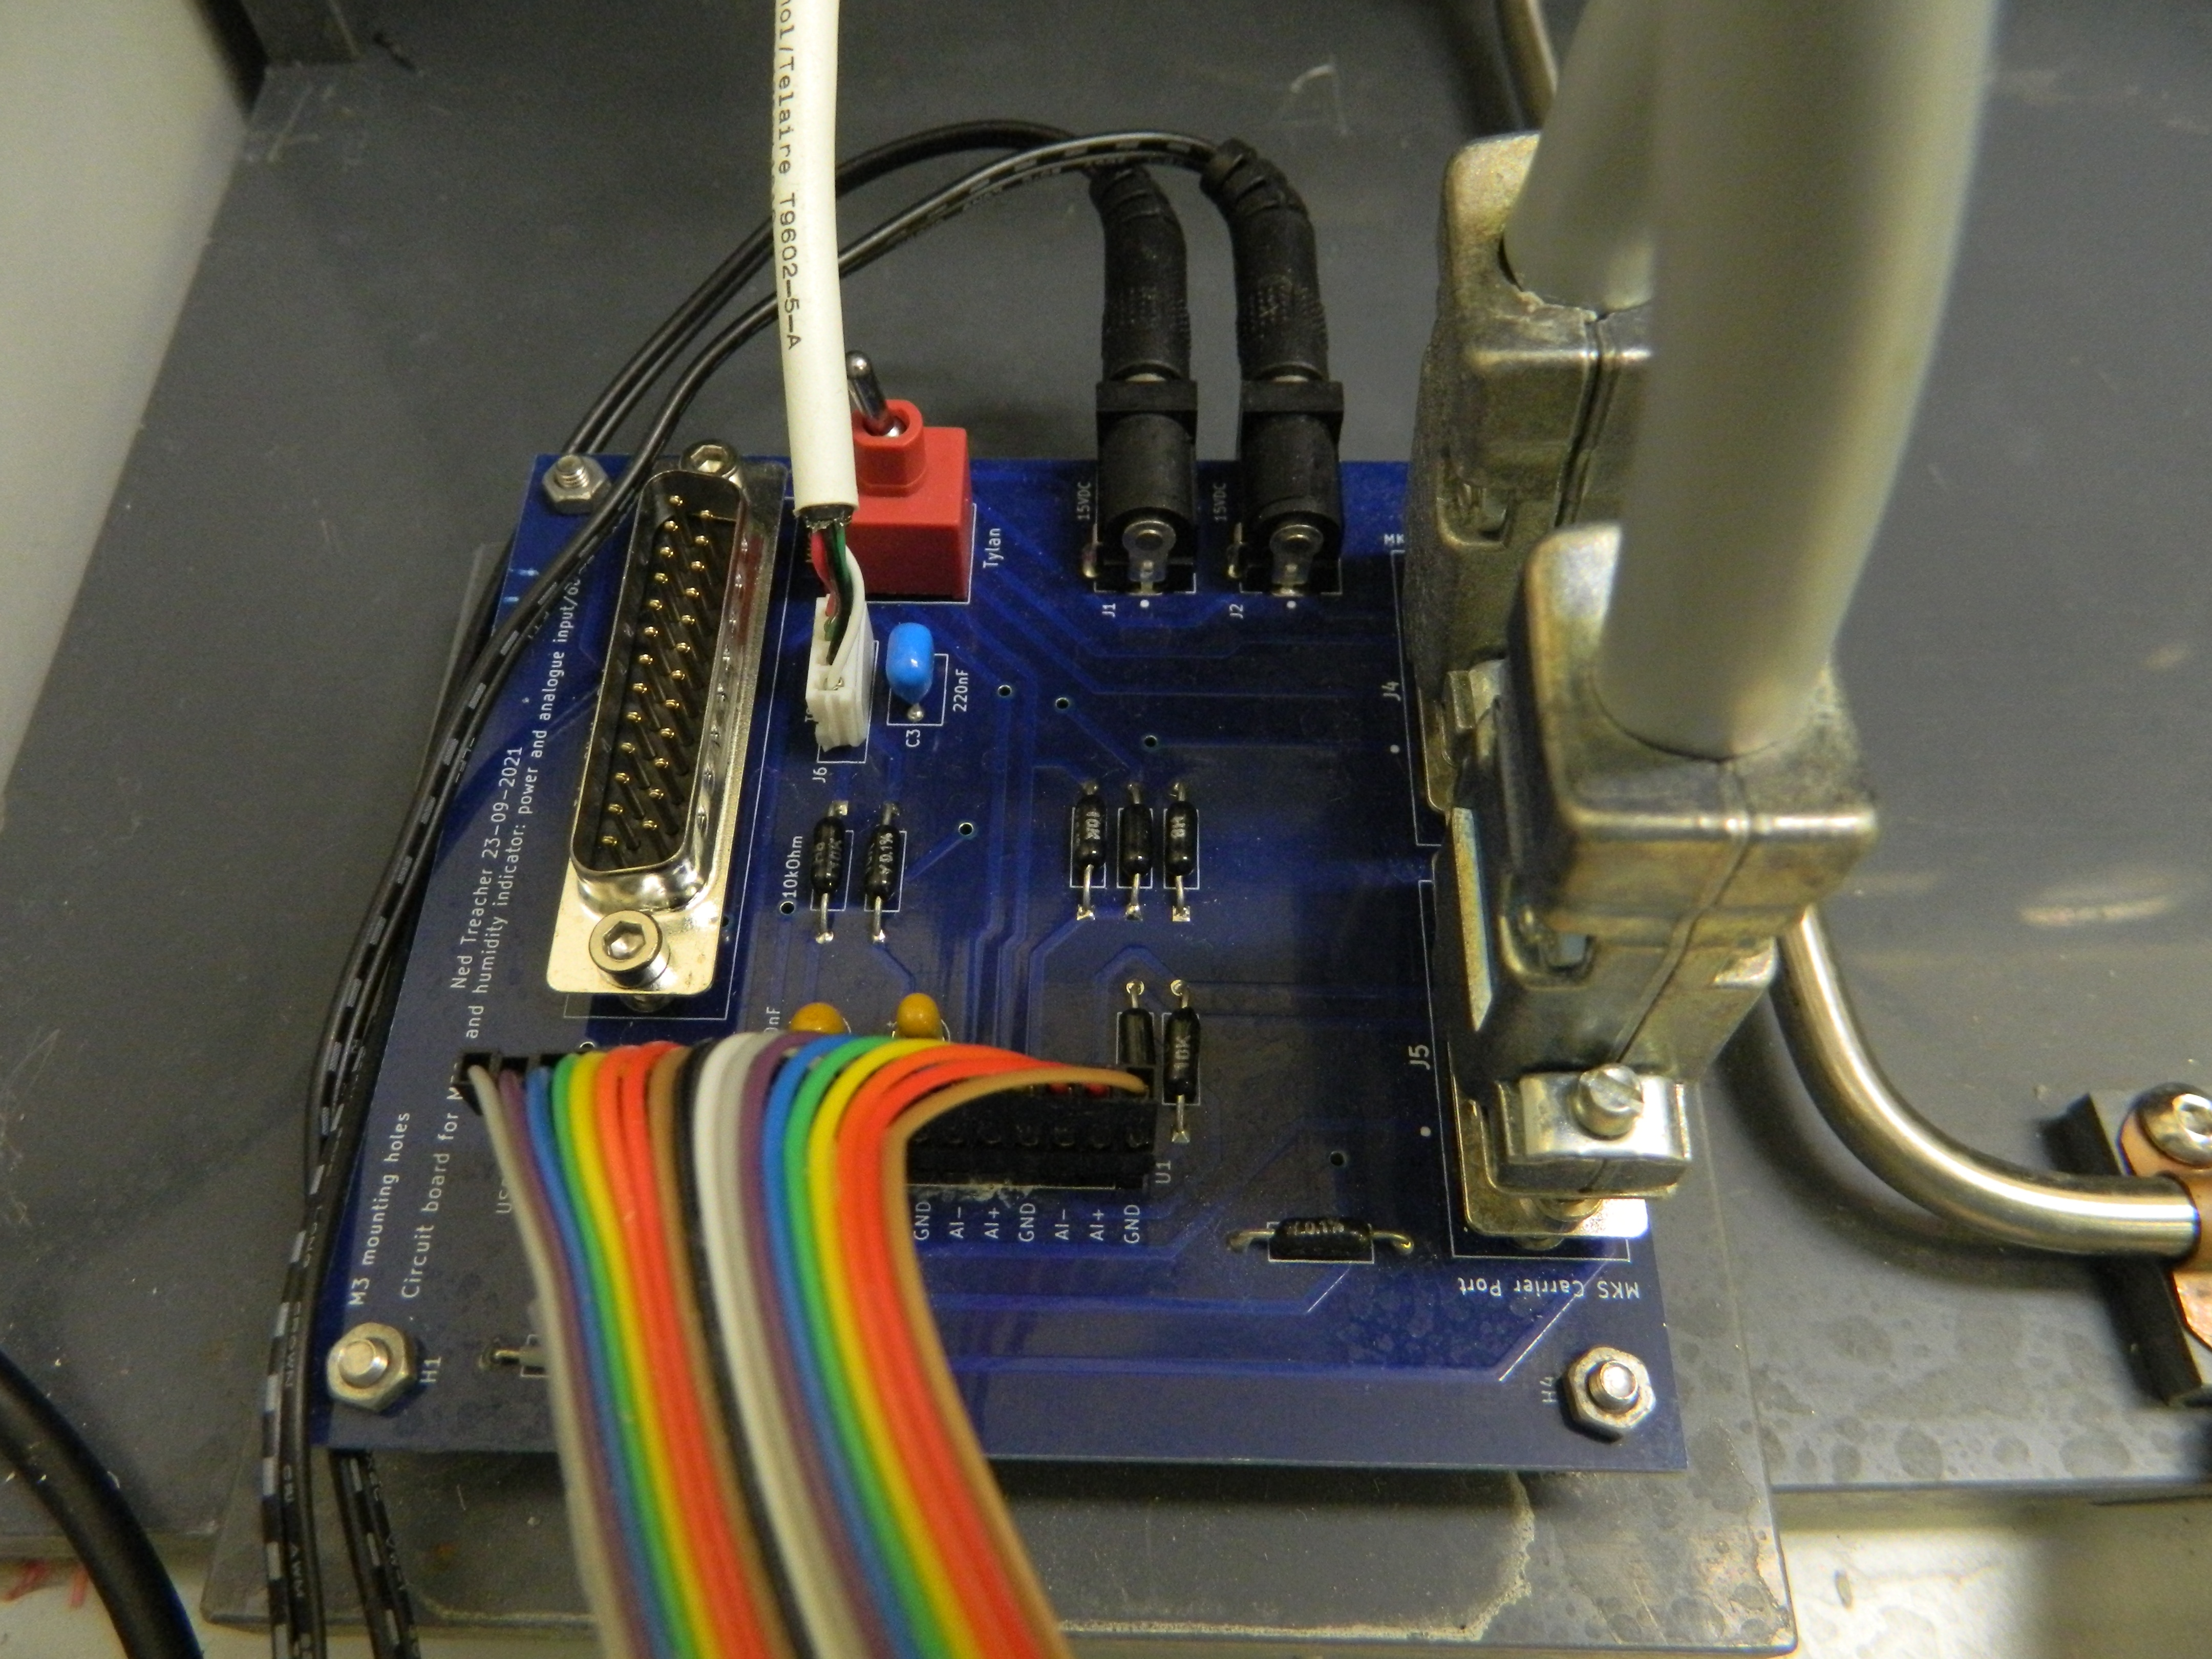
\includegraphics{figures/ch5/low_flow_config.png}

}

}

\subcaption{\label{fig-low-flow}}
\end{minipage}%
%
\begin{minipage}[t]{0.05\linewidth}

{\centering 

~

}

\end{minipage}%
%
\begin{minipage}[t]{0.47\linewidth}

{\centering 

\raisebox{-\height}{

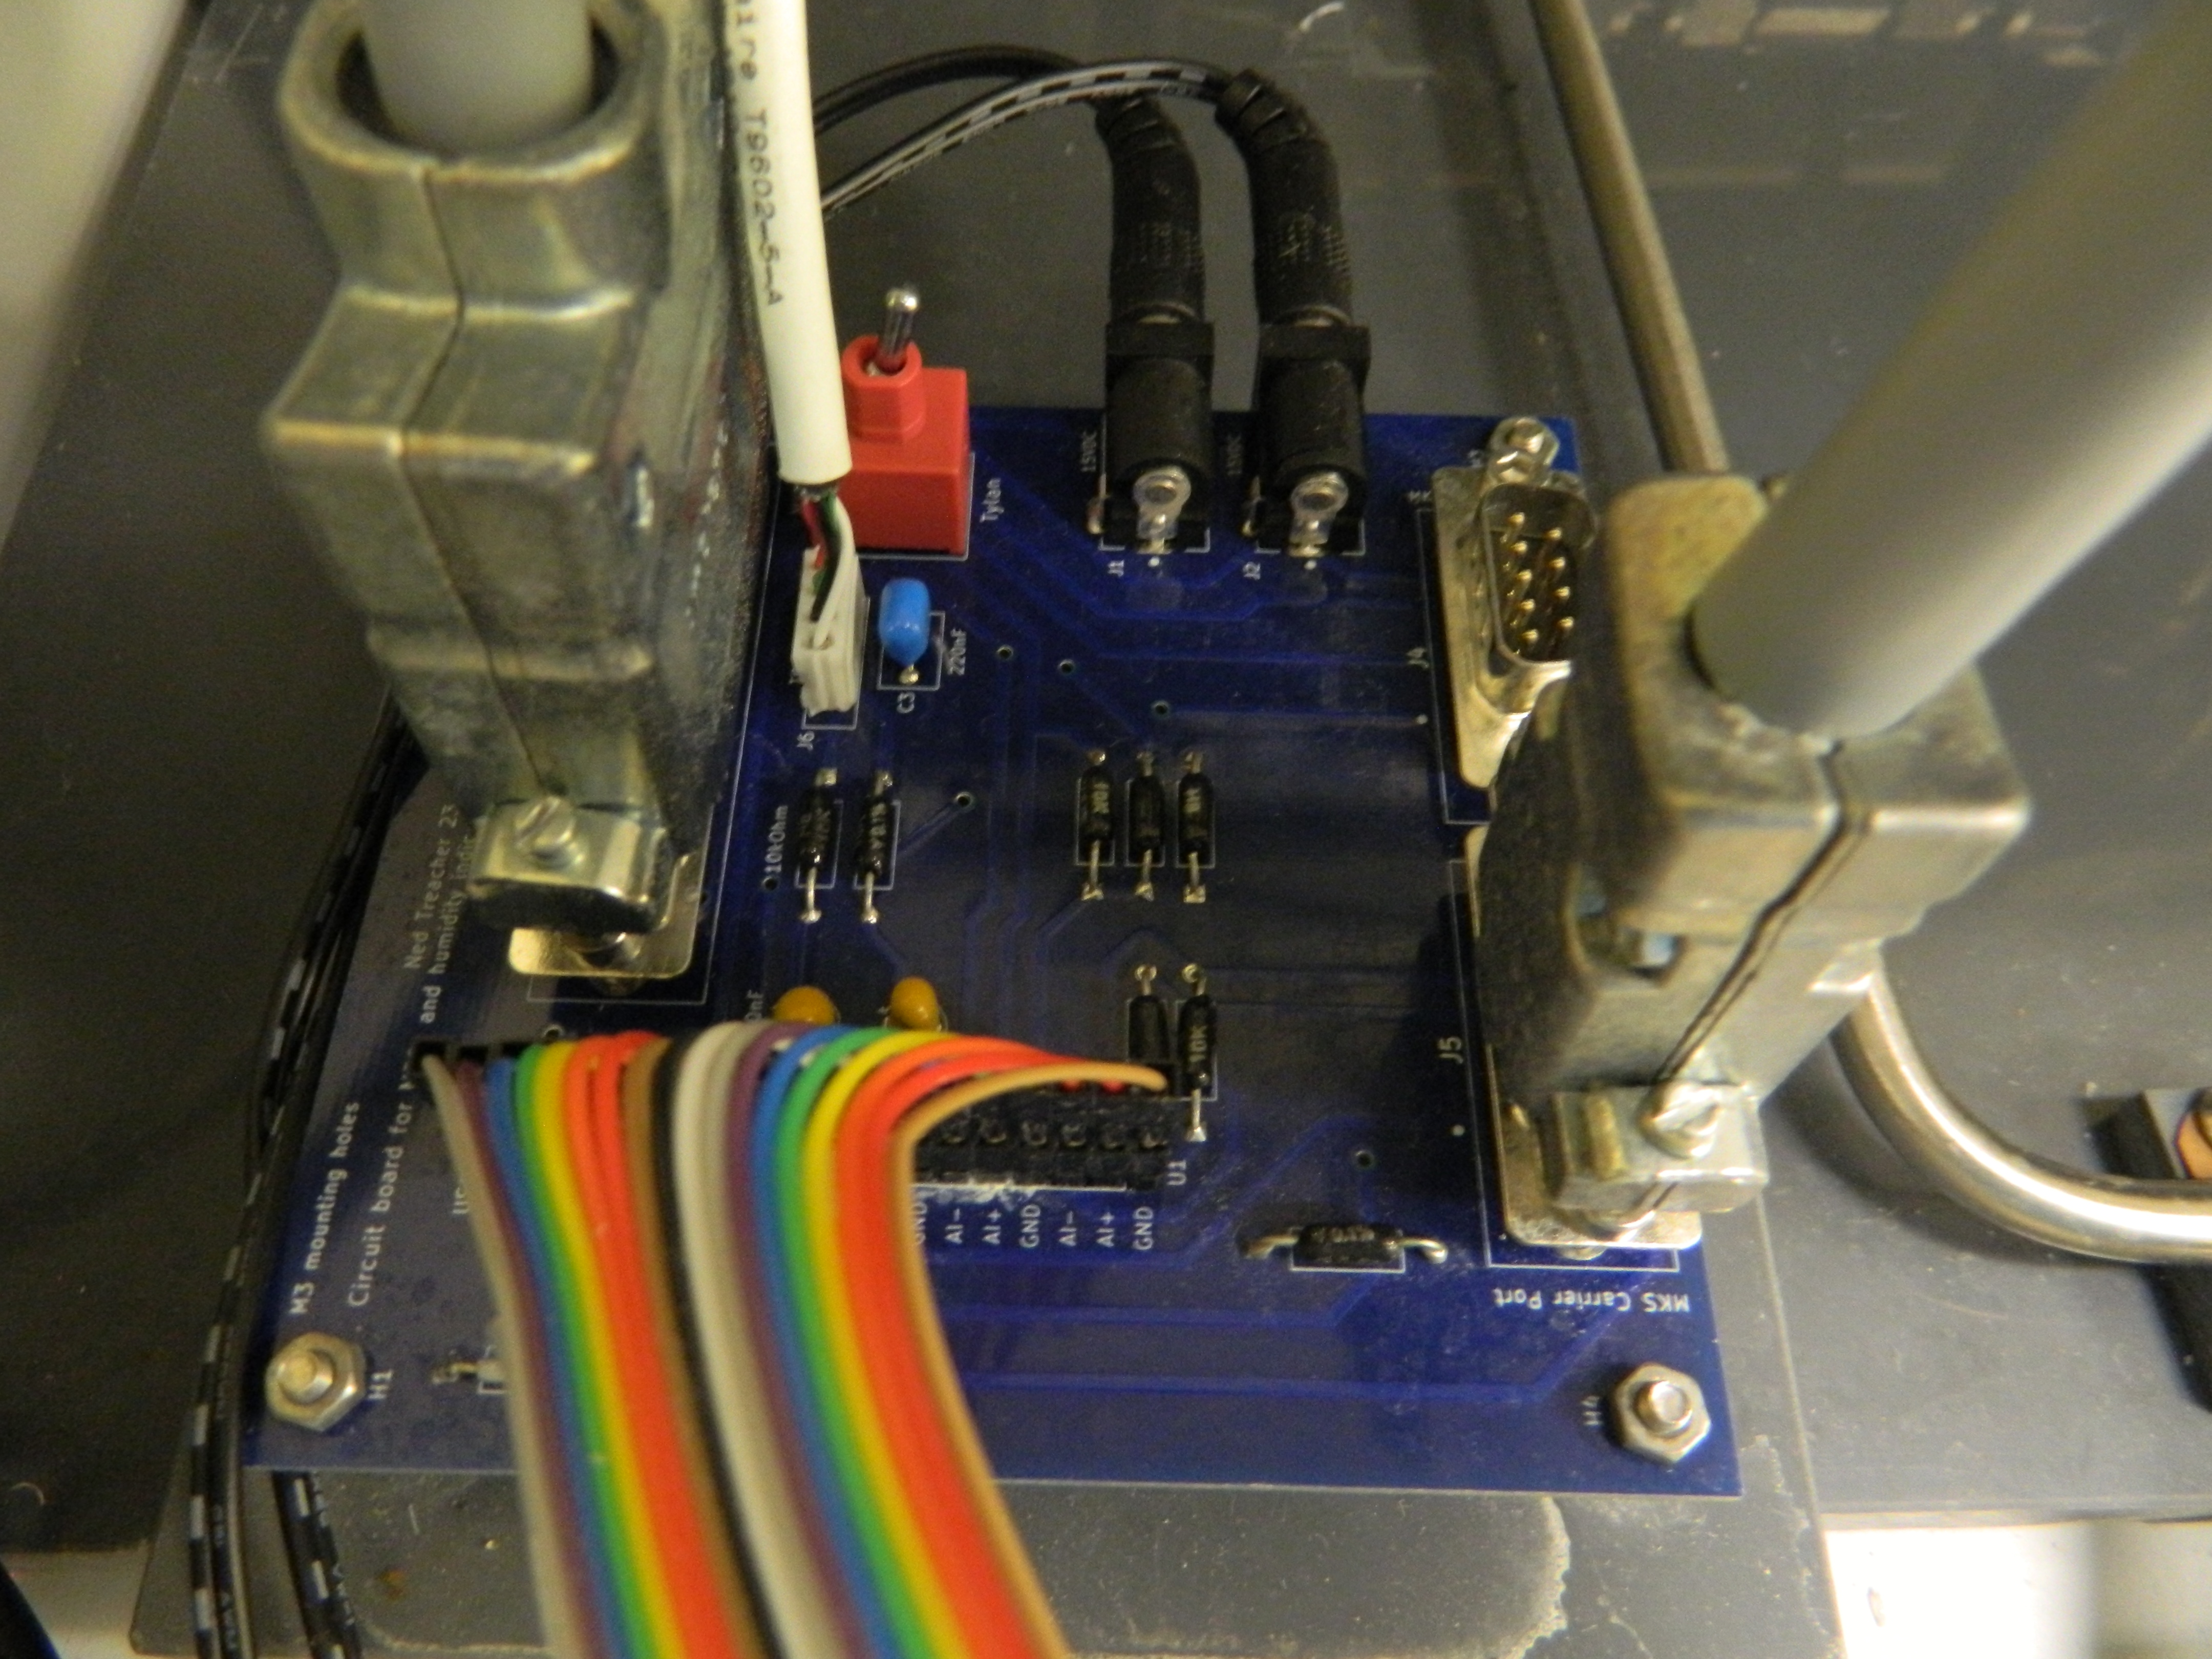
\includegraphics{figures/ch5/high_flow_config.png}

}

}

\subcaption{\label{fig-high-flow}}
\end{minipage}%

\caption{\label{fig-vapour-sensor-pcb}Images of the vapour delivery
control system circuit board, where (a) shows the low-flow configuration
and (b) shows the high-flow configuration. Components are labelled as
follows: (1) 9-pin carrier line port, (2) 9-pin dilution line port, (3)
dilution port switch (determines which dilution line port is active),
(4) 25-pin dilution line port. In (a), the 500 sccm full-scale MFC is
connected at the 25-pin dilution line port, the 200 sccm full-scale MFC
is connected at the 9-pin carrier line port and the red dilution port
switch is towards ``Tylan'' (to the right). In (b), the 200 sccm
full-scale MFC is connected at the 9-pin dilution line port, the 20 sccm
full-scale MFC is connected at the 9-pin carrier line port and the red
dilution port switch is towards ``MKS'' (to the left).}

\end{figure}

\begin{figure}

{\centering 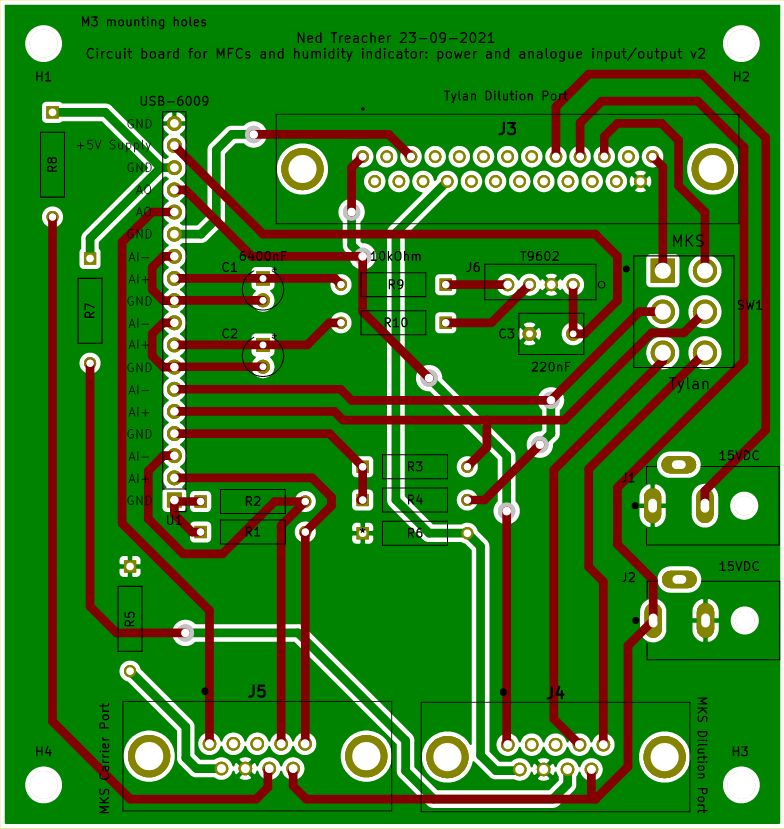
\includegraphics[width=0.95\textwidth,height=\textheight]{figures/ch5/current_PCB.png}

}

\caption{\label{fig-current-pcb-design}Circuit board schematic for
controlling and monitoring both the mass flow controllers and the
relative humidity and temperature sensor. The relative humidity and
temperature sensor is connected to the circuit board via the T9602
footprint. The mass flow controllers connect to the board in two
configurations. The first (``high-flow'') configuration has the Tylan
dilution and MKS carrier ports connected, with switch SW1 in the Tylan
direction. The second (``low-flow'') configuration has both MKS ports
connected, with switch SW1 connected in the MKS direction. Resistors
R1-R6 are all 10 kOhm, while R7-R8 are both 0 Ohm. The circuit board was
designed using the KiCad Layout Editor.}

\end{figure}

The control circuit board used to connect the mass flow controllers and
relative humidity and temperature indicator to the NI USB-6009 is shown
in Figure~\ref{fig-vapour-sensor-pcb}. Only one mass flow controller can
be set to provide flow to a specific line, and so only two mass flow
controllers can be operational simultaneously during testing with the
vapour delivery system. The control circuit board allows the user to set
which two mass flow controllers are to be used during a specific test
run. Figure~\ref{fig-high-flow} shows the ``high-flow'' configuration,
where the 500 sccm full-scale MFC is connected to the dilution line and
the 200 sccm full-scale MFC is connected to the carrier line.
Figure~\ref{fig-low-flow} shows the ``low-flow'' configuration, where
the 200 sccm full-scale MFC is connected to the dilution line and the 20
sccm full-scale MFC is connected to the carrier line. The design for the
circuit board is shown in Figure~\ref{fig-current-pcb-design}, showing
the pinout to the USB-6009 and the various components used to connect
the MFCs, relative humidity indicator, and the power supply for the
MFCs.

\hypertarget{software}{%
\subsubsection*{Software}\label{software}}
\addcontentsline{toc}{subsubsection}{Software}

Two LabView Virtual Instruments (VIs) were adapted from pre-existing VIs
for operating the mass flow controllers and monitoring vapour flow into
the device chamber, as well as monitoring temperature and humidity in
the vapour delivery system's manifold. These VIs were named
``vapour-sensor-basic.vi'' and ``temp-and-humidity-basic.vi''. A third
VI was developed in parallel which combined the first two Virtual
Instruments and allowed the user to set a sequence of values for the
output flow from the mass flow controllers before an experimental run.
This VI was named ``vapour-sensor-sequence-timestamped.vi''. Flow rate,
relative humidity and temperature data were then saved as .lvm files.
The LabView VIs described here are available on request.

\hypertarget{sec-vapour-system-design}{%
\section{Design}\label{sec-vapour-system-design}}

\hypertarget{initial-design}{%
\subsection{Initial Design}\label{initial-design}}

\begin{figure}

{\centering 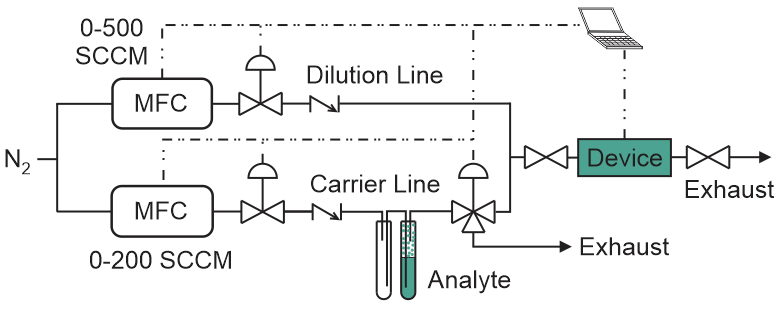
\includegraphics[width=1\textwidth,height=\textheight]{figures/ch5/PID_V0.png}

}

\caption{\label{fig-original-pid}P\&ID of the original vapour delivery
system}

\end{figure}

\begin{figure}

\begin{minipage}[t]{0.38\linewidth}

{\centering 

\raisebox{-\height}{

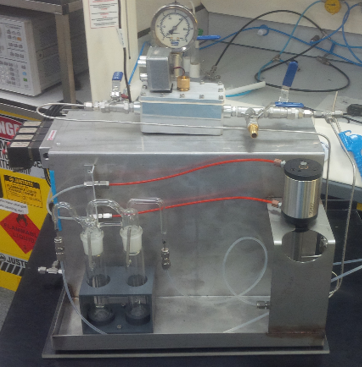
\includegraphics{figures/ch5/original_system_front.png}

}

}

\subcaption{\label{fig-original-front}}
\end{minipage}%
%
\begin{minipage}[t]{0.05\linewidth}

{\centering 

~

}

\end{minipage}%
%
\begin{minipage}[t]{0.57\linewidth}

{\centering 

\raisebox{-\height}{

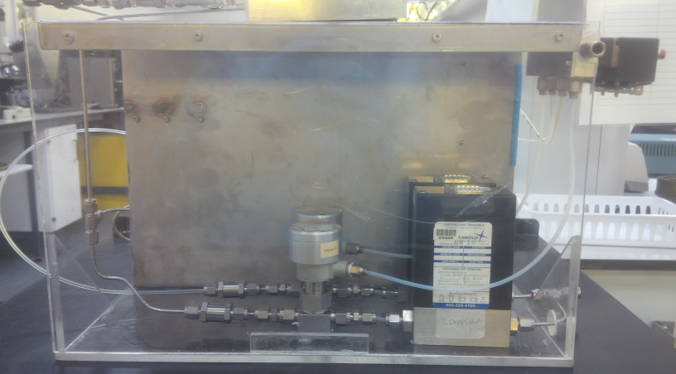
\includegraphics{figures/ch5/original_system_back.png}

}

}

\subcaption{\label{fig-original-back}}
\end{minipage}%

\caption{\label{fig-original-setup}The original vapour delivery system
setup, where (a) shows the front of the system, including the device
chamber, analyte bottles and four-way valve, and (b) shows the back of
the system, including the mass flow controllers and solenoid valves.}

\end{figure}

\begin{figure}

{\centering \includegraphics[width=0.55\textwidth,height=\textheight]{figures/ch5/original_pcb.png}

}

\caption{\label{fig-original-pcb}The control circuit board for the
original vapour delivery system.}

\end{figure}

The initial design of the vapour delivery system, as shown in
Figure~\ref{fig-original-pid}, was relatively simple. No reference
sensors were included in the setup, and only one channel could be
characterised without opening the chamber and changing the position of
the device. However, as constructed it worked well as a self-contained
system, which was able to deliver vapour to a device channel while
measuring current across the channel. The original system is shown in
Figure~\ref{fig-original-setup}, and the circuit board used to control
it is shown in@fig-original-pcb A 500 sccm full-range MFC (Tylan) was
placed on the dilution line, and a 200 sccm full-range MFC (Tylan) was
placed on the carrier line. A glass container for analyte was present on
the carrier line, with a vapour trap upstream to collect any backflow.
The vapour trap was removed in later iterations due to the presence of a
check valve to prevent backflow. The device chamber and mass flow
controllers were connected to a laptop and an Agilent 4156C
semiconductor parameter analyser and controlled using LabView.

\hypertarget{sec-vapour-system-design-1}{%
\subsection{Stage I Design}\label{sec-vapour-system-design-1}}

\begin{figure}

{\centering 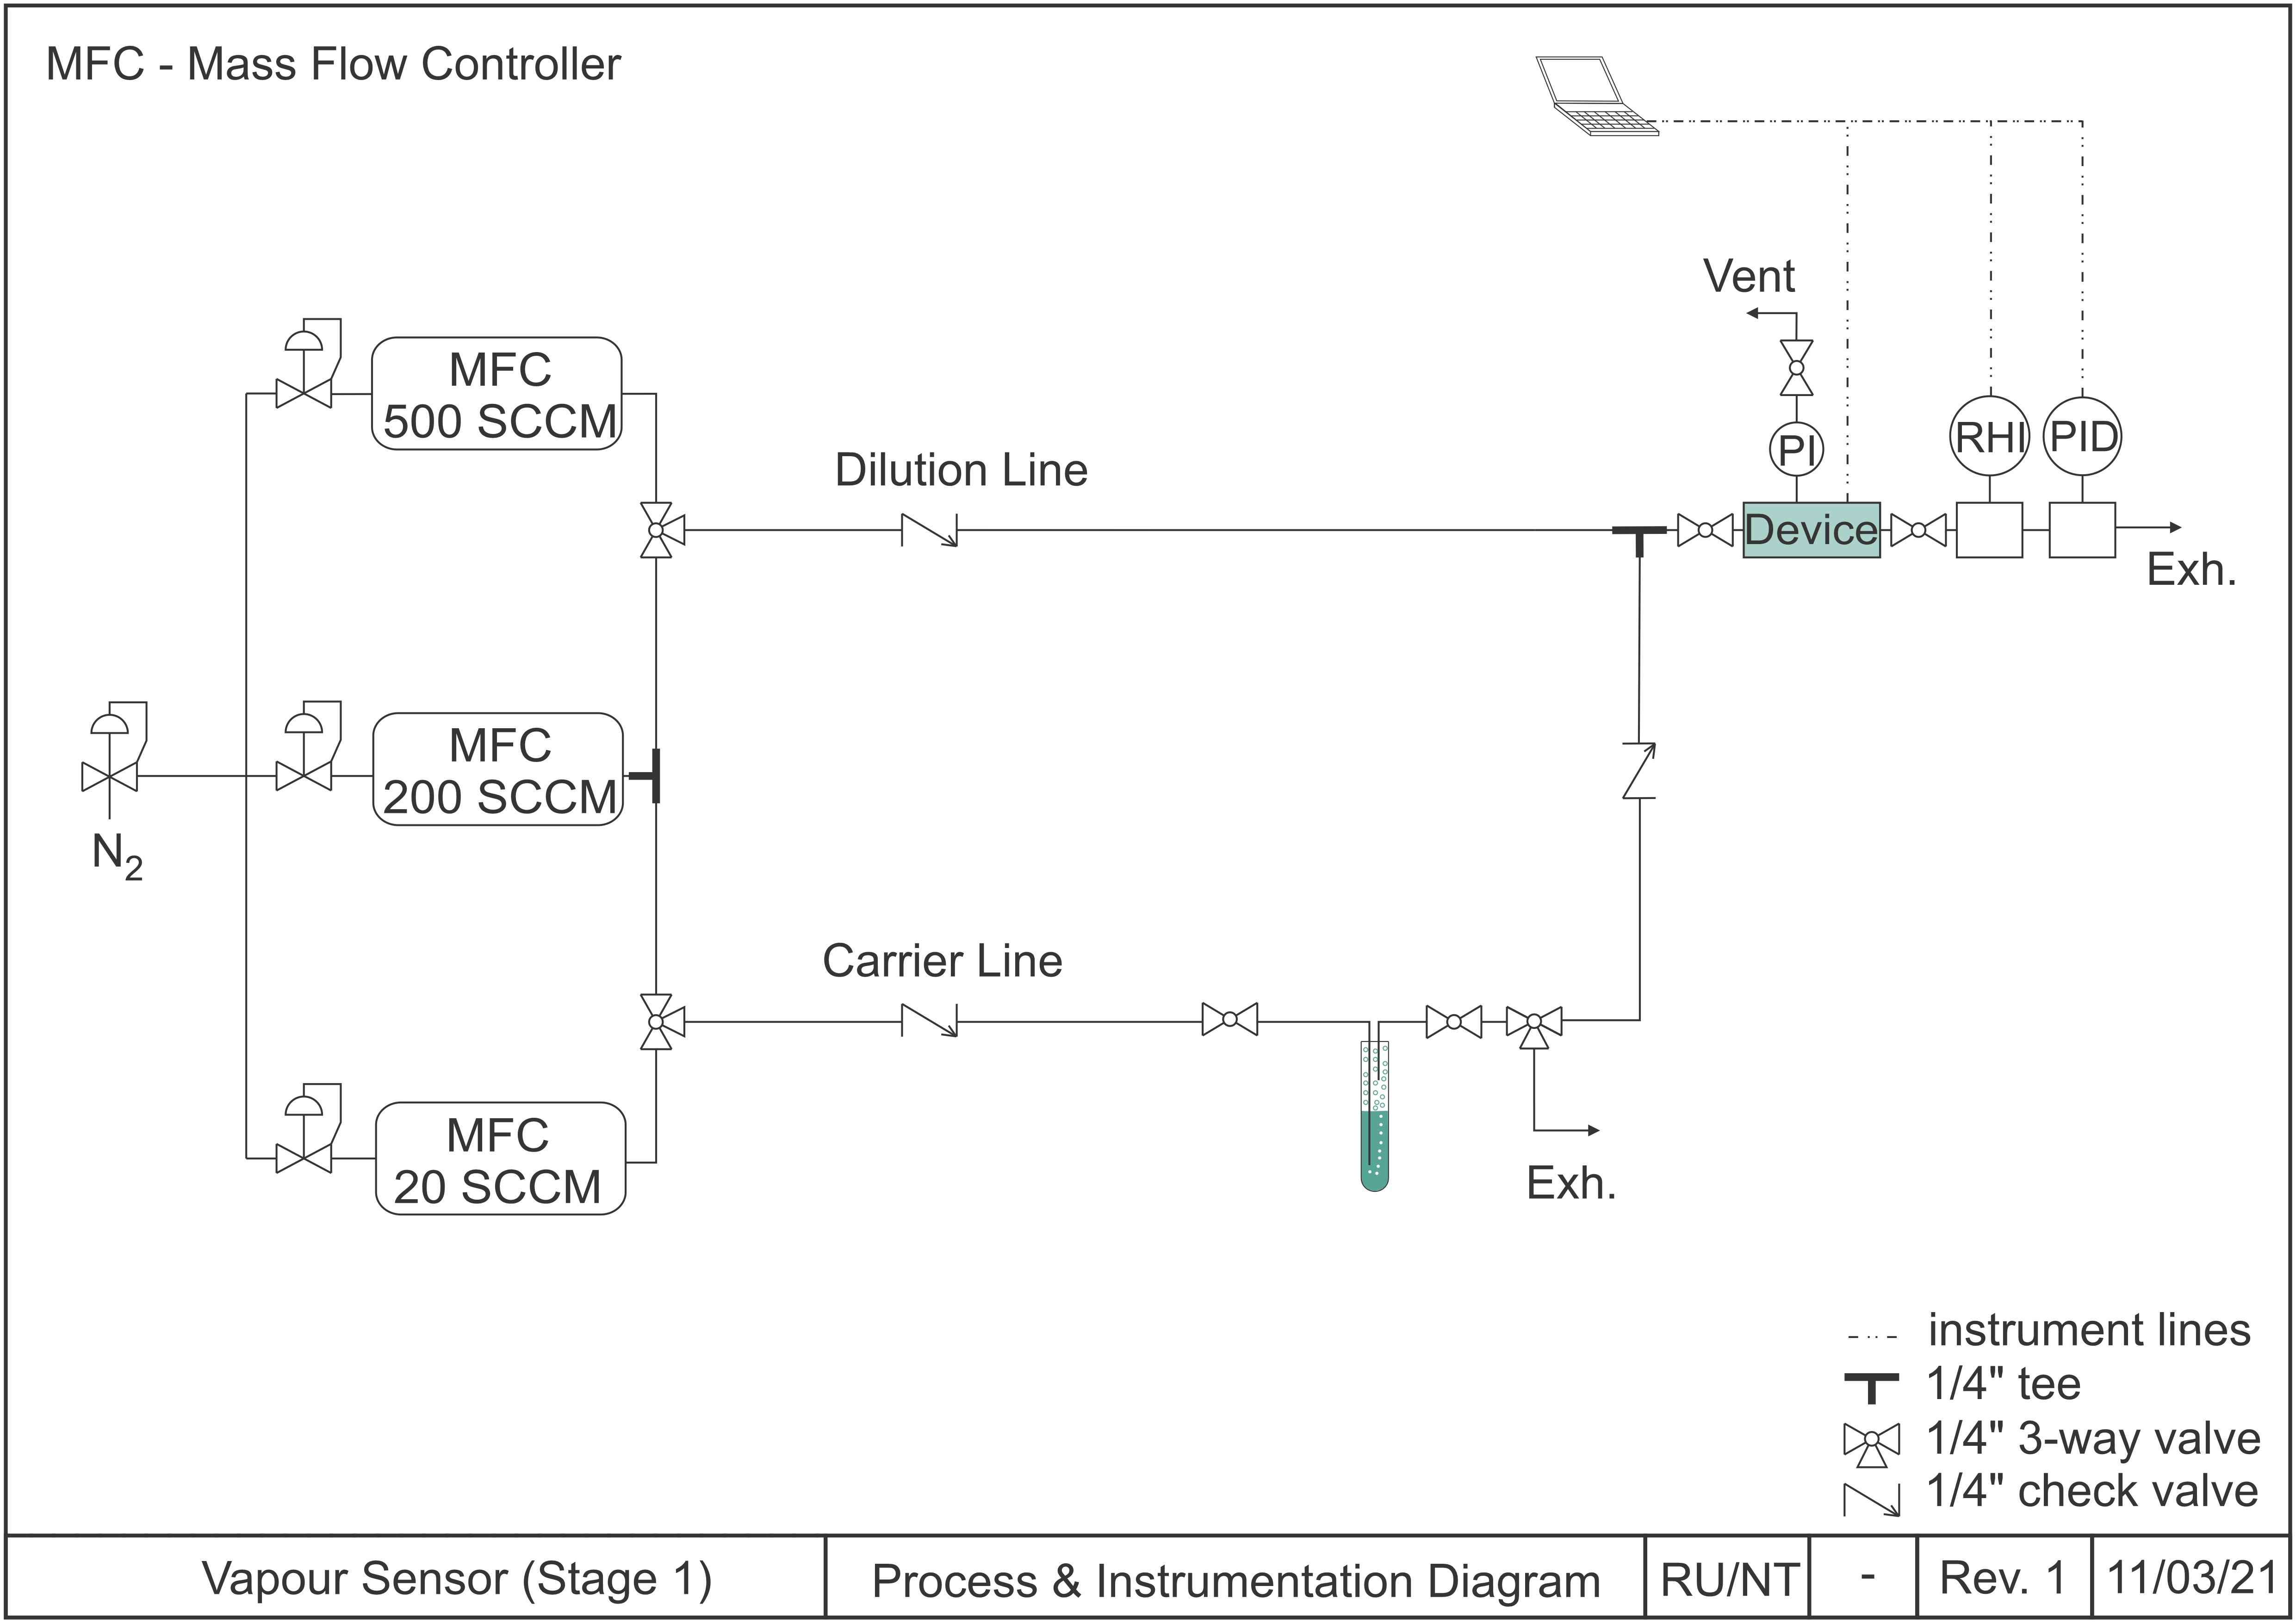
\includegraphics[width=1\textwidth,height=\textheight]{figures/ch5/PID_V1.png}

}

\caption{\label{fig-stage-1-pid}P\&ID of the Stage I vapour delivery
system.}

\end{figure}

\begin{figure}

{\centering 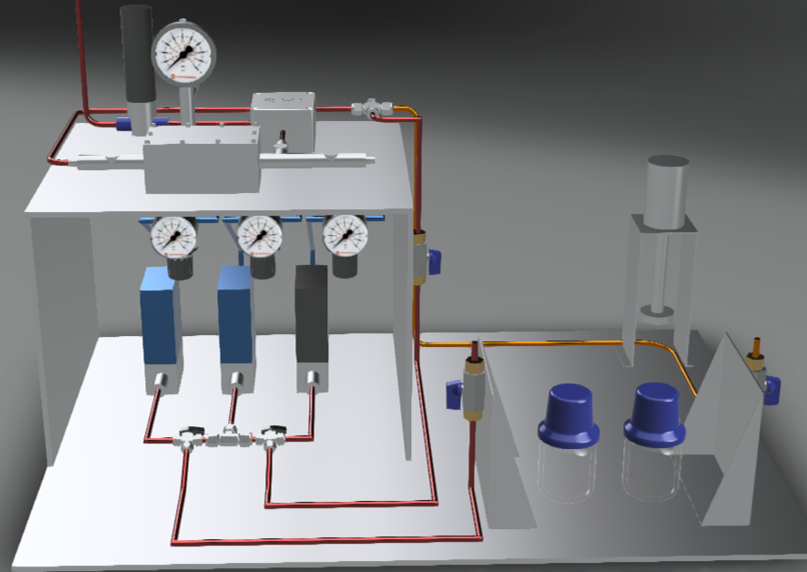
\includegraphics[width=1\textwidth,height=\textheight]{figures/ch5/cad_V1.png}

}

\caption{\label{fig-stage-1-cad}Conceptual 3D Model of Stage I vapour
delivery system. The model was made in Autodesk 360 by Alex Puglisi,
School of Chemical and Physical Sciences, Te Herenga Waka - Victoria
University of Wellington.}

\end{figure}

The first stage of the vapour delivery system redesign, as shown in
Figure~\ref{fig-stage-1-pid} and Figure~\ref{fig-stage-1-cad} was
implemented in Nov 2021. This system introduced the ability to use a 20
sccm full-range MFC (MKS Instruments) for carrier line flow and a 200
sccm full-range MFC (MKS Instruments) for either carrier or dilution
line flow, to give better control when using low flow rates. The
reference sensors were also implemented, with each sensor connected in
parallel to the chamber exhaust. Through testing the system with ethanol
and acetone as analytes, the following issues with this implementation
of the setup were identified:

\begin{itemize}
\item
  With the system connected to the lab supply of nitrogen, pressure
  changes in the line due to nitrogen use elsewhere in the lab impacted
  the pressure at the MFCs and the flow through the lines.
\item
  The pressure indicator used for the device chamber had a much wider
  range than the pressure reached before nitrogen began to leak out of
  the PVC tubing; this meant pressure changes in the chamber, resulting
  from closing the exit valves while nitrogen flow entered the chamber,
  did not register on the indicator.
\item
  The PID responded unexpectedly slowly to changes in vapour
  concentration in the chamber. For example, after acetone or ethanol
  vapour had been run through the chamber, running clean nitrogen
  through the system for 3 hours was required before the PID returned to
  a constant baseline reading.
\item
  There was no way to ensure the device chamber was free of analyte
  vapour before an experimental run aside from running nitrogen through
  the dilution line. After prolonged use, condensed analyte was
  sometimes visible in the PVC lines of the delivery system.
\end{itemize}

These issues, along with various minor structural and design issues,
were addressed in the second-stage implementation of the system.

\hypertarget{stage-ii-design}{%
\subsection{Stage II Design}\label{stage-ii-design}}

\begin{figure}

{\centering 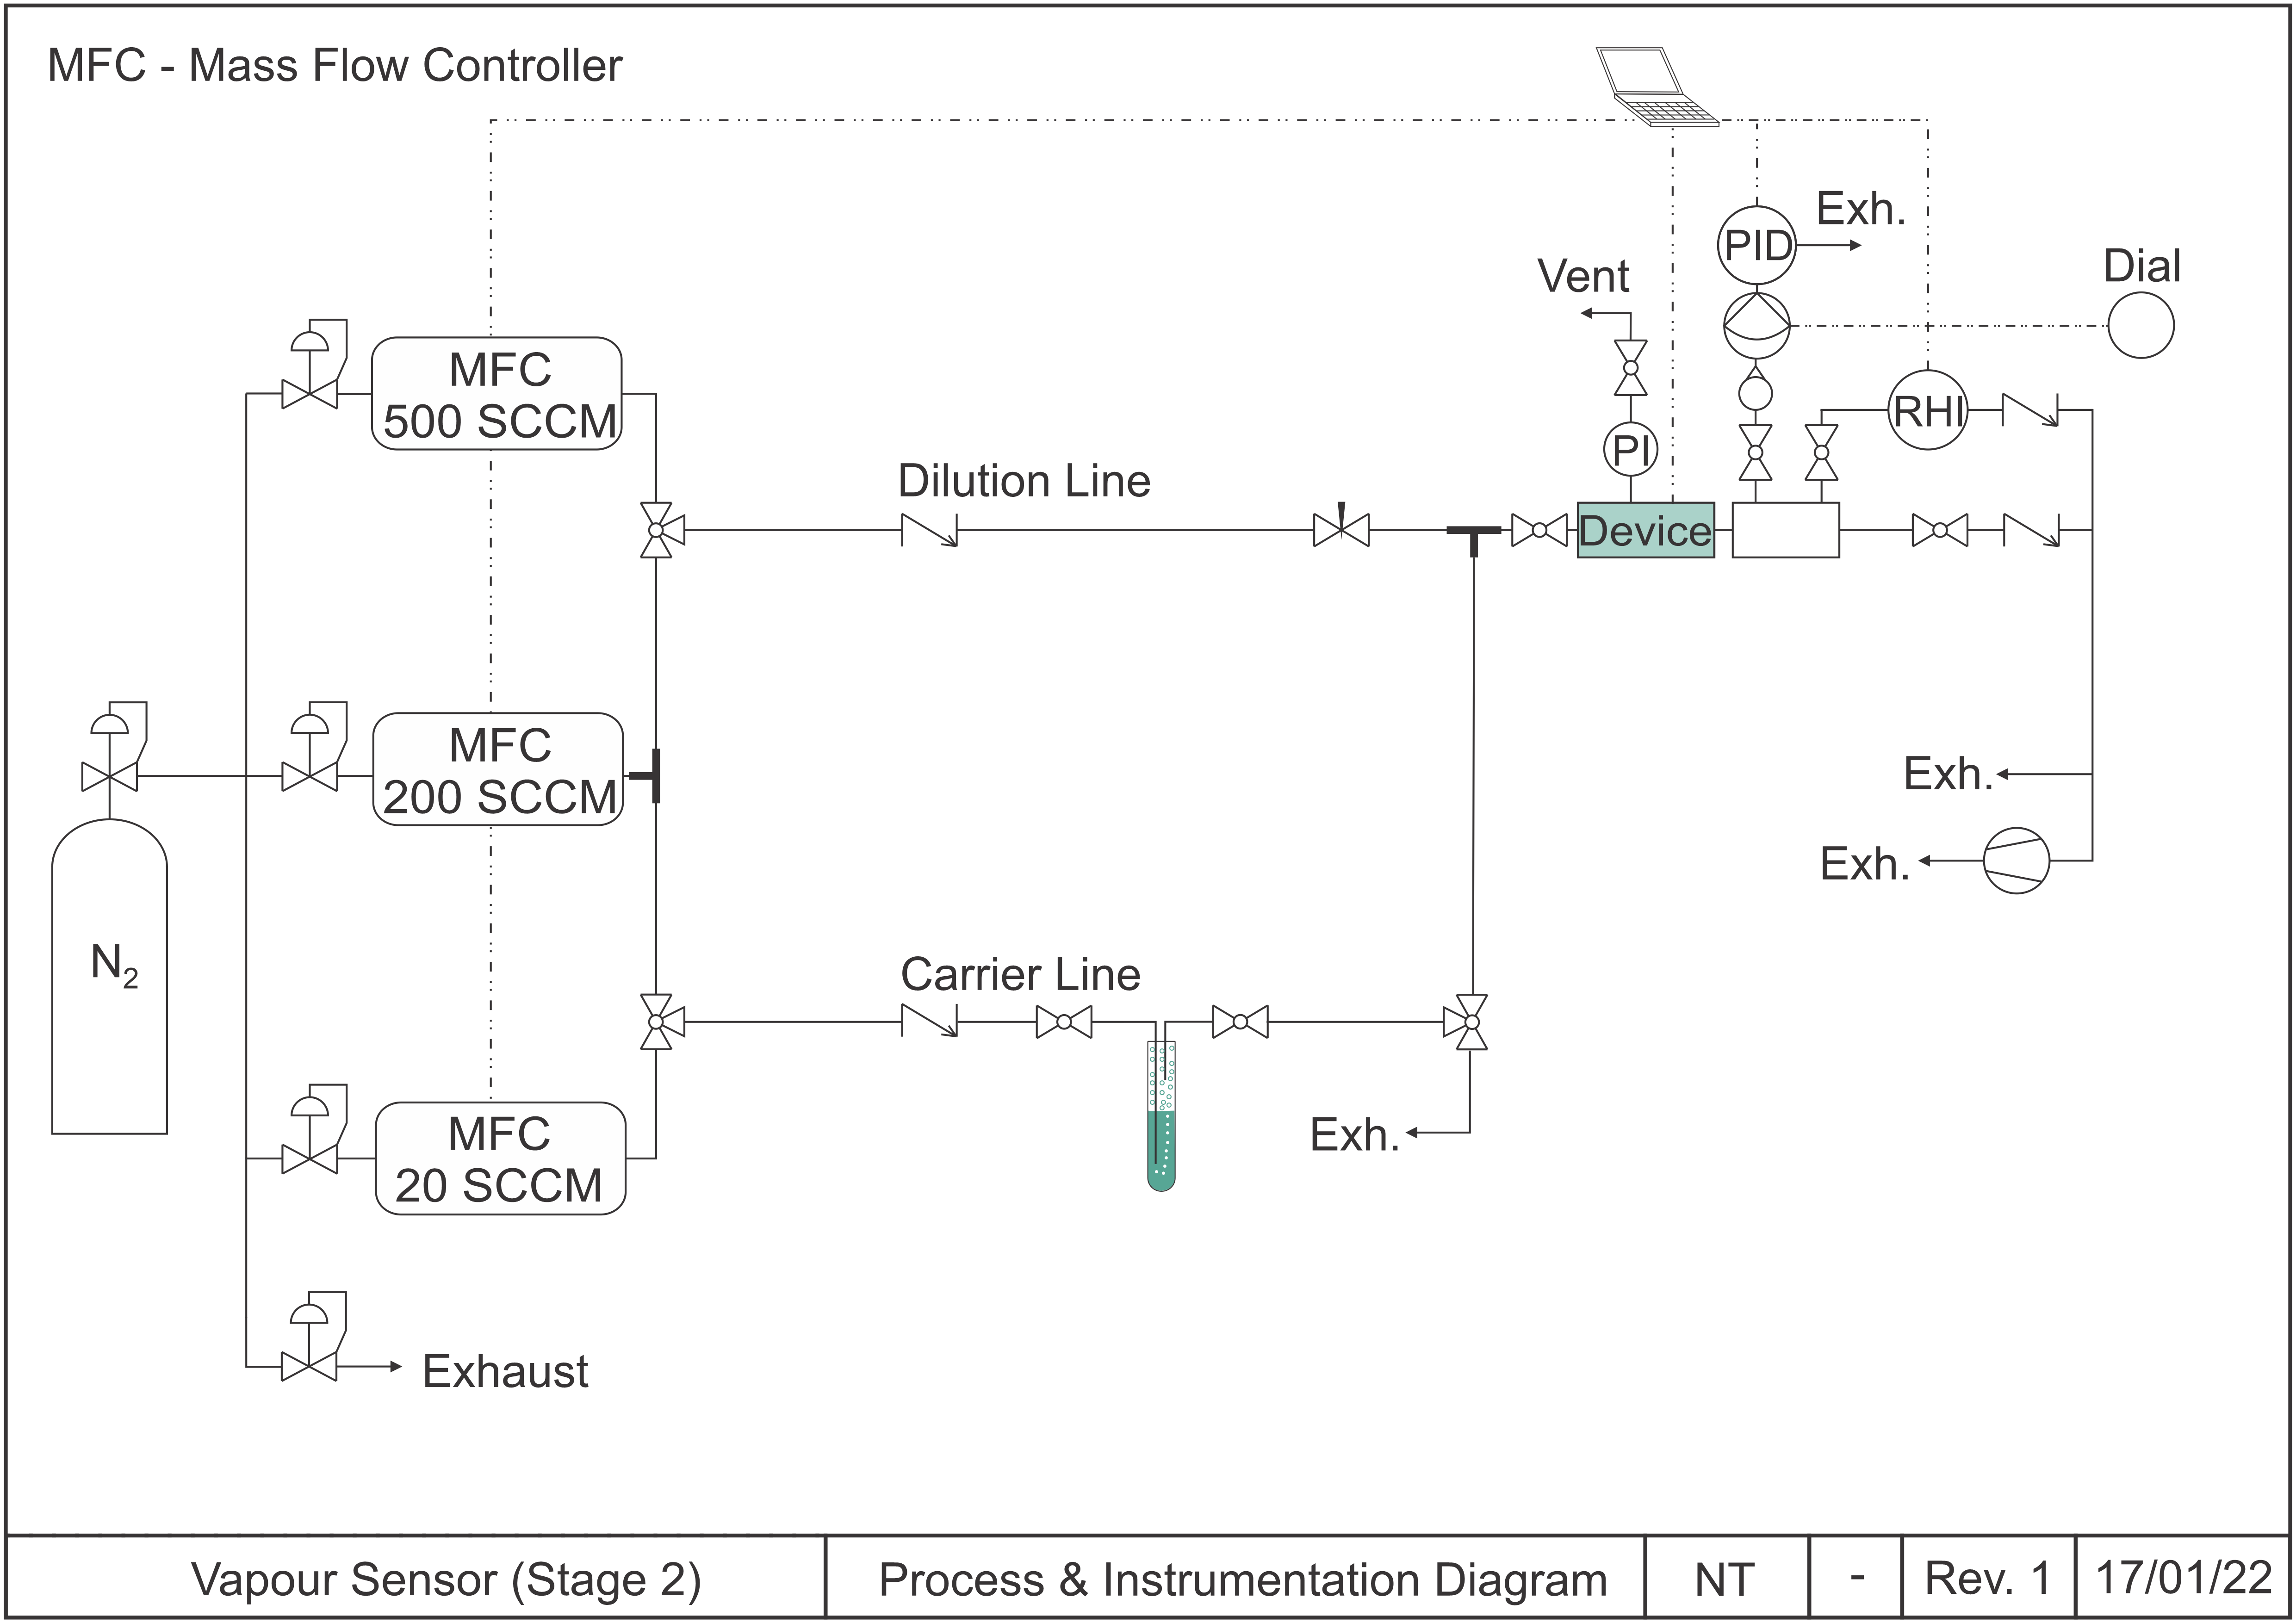
\includegraphics[width=1\textwidth,height=\textheight]{figures/ch5/PID_V2.png}

}

\caption{\label{fig-stage-2-pid}Process \& instrumentation diagram
(P\&ID) of the second-stage design for the vapour delivery system.}

\end{figure}

Figure~\ref{fig-stage-2-pid} gives an overview of the second-stage
design for the vapour delivery system setup. This stage of the redesign
was implemented between Jan and May 2022. Changes from the first stage
included:

\begin{itemize}
\item
  The addition of a N\(_2\) cylinder (152D size) as the source of
  nitrogen for the system to replace the lab supply.
\item
  A pressure indicator with a lower pressure range was used, which could
  register pressure changes within the device chamber.
\item
  A chamber manifold was placed before the exhaust with outlets into the
  PID and RHI.
\item
  A micro diaphragm pump was introduced between the manifold and PID to
  supply the PID with vapour from the chamber, and a flowmeter was
  placed before the pump to measure the flow rate out of the chamber to
  the PID. The PID was then seen to respond quickly to system changes
  (discussed further in Section~\ref{sec-calibration}).
\item
  A piece of PVC tubing was placed at the PID outlet to limit air from
  the fumehood entering the PID when the micropump was off.
\item
  Valves were placed before all system components so that the device
  chamber and post-analyte bottle carrier line could be evacuated with a
  roughing pump without potentially affecting components.
\item
  Check valves were placed at the exhaust to prevent backflow from the
  roughing pump into the delivery system.
\end{itemize}

These changes largely addressed the issues identified in
Section~\ref{sec-vapour-system-design-1}.

\hypertarget{sec-calibration}{%
\section{Calibration and Measurements of Vapour
Flow}\label{sec-calibration}}

\hypertarget{sec-flow-calibration}{%
\subsection{Chamber Flow Calibration}\label{sec-flow-calibration}}

\begin{figure}

{\centering 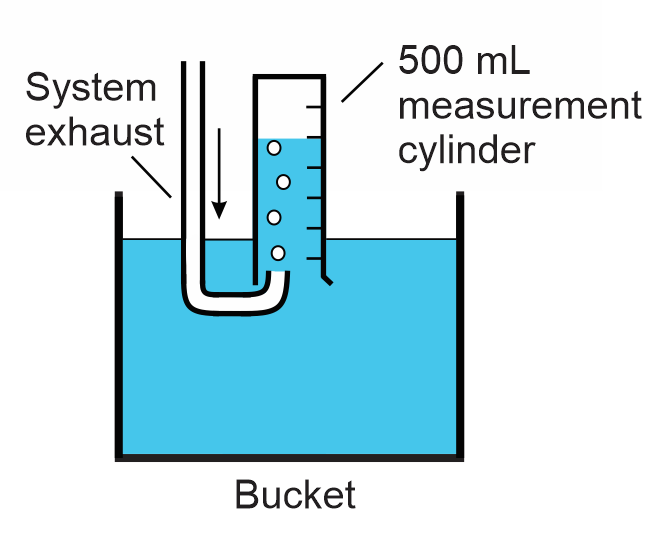
\includegraphics[width=0.45\textwidth,height=\textheight]{figures/ch5/water_displacement.png}

}

\caption{\label{fig-water-displacement}Setup for calibration of mass
flow controllers using the water displacement method.}

\end{figure}

A water displacement test was carried out to determine the relationship
between the flow rate measured by the mass flow controllers and the
actual flow rate passing through the chamber. All valves were set so
that both the dilution and carrier lines followed a single path. Both
these paths went through the device chamber and out through the system
exhaust. An empty analyte bottle was placed on the carrier line. The
system exhaust was placed into a bucket filled with tap water, with the
outlet sitting beneath an upturned 500 mL measurement cylinder, as
pictured in Figure~\ref{fig-water-displacement}. The cylinder was used
to measure the volume of displaced water over time, which is equivalent
to the rate of change of nitrogen volume entering the cylinder from the
exhaust. As leaks in the manifold and exhaust line were not detected
when leak testing with bubble solution, it can be safely assumed that
the rate at which nitrogen exits the exhaust is equivalent to the
nitrogen flow rate through the device chamber.

\begin{figure}

\begin{minipage}[t]{0.47\linewidth}

{\centering 

\raisebox{-\height}{

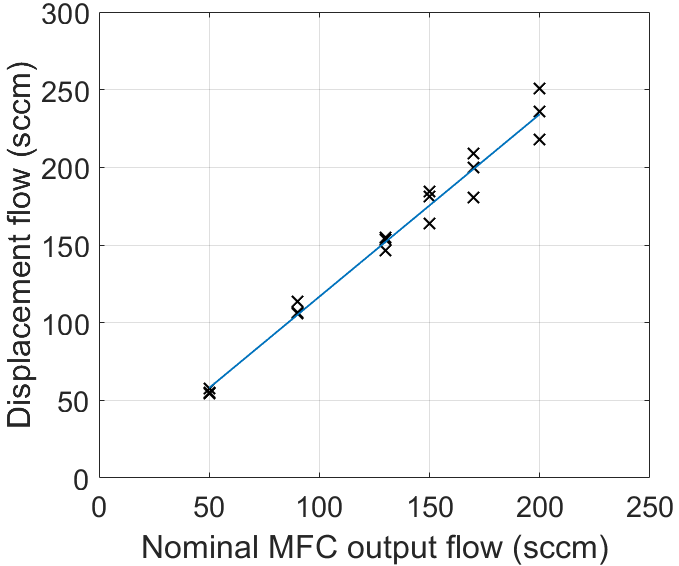
\includegraphics{figures/ch5/200sccmMFC_carrierline_thruchamber.png}

}

}

\subcaption{\label{fig-200-MFC-curve}}
\end{minipage}%
%
\begin{minipage}[t]{0.05\linewidth}

{\centering 

~

}

\end{minipage}%
%
\begin{minipage}[t]{0.47\linewidth}

{\centering 

\raisebox{-\height}{

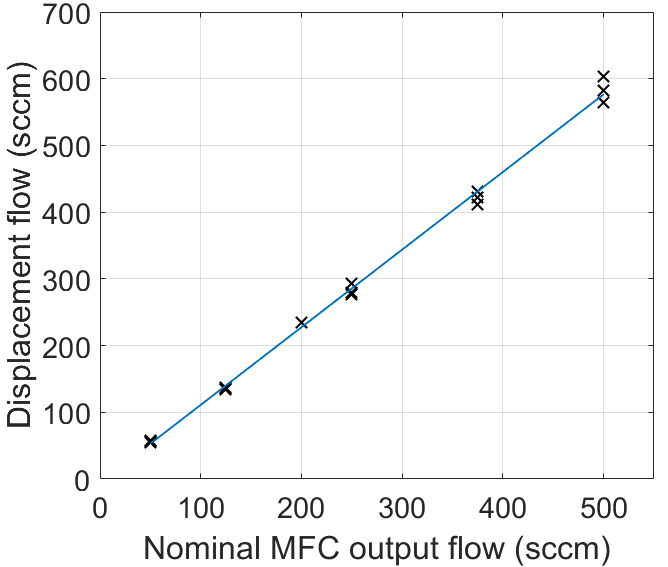
\includegraphics{figures/ch5/500sccmMFC_dilutionline_thruchamber.png}

}

}

\subcaption{\label{fig-500-MFC-curve}}
\end{minipage}%

\caption{\label{fig-MFC-calibration-curves}Calibration curves for the
200 sccm full-scale MFC through the carrier line (a) and the 500 sccm
full-scale MFC through the dilution line (b).}

\end{figure}

The time taken to displace a fixed volume of water was measured three
times for a series of constant flow rates, both for the 200 sccm MFC
(MKS) on the carrier line and the 500 sccm MFC (Tylan) on the dilution
line. The displacement flow rate corresponding to each measurement could
then be found by dividing volume by time. These measurements, of
displacement flow relative to nominal flow through the MFC, are shown in
Figure~\ref{fig-MFC-calibration-curves}. The flow through the chamber
was offset from the nominal flow reading from the mass flow controllers,
with a strong linear relationship between the two measurements. A linear
least-squares fit was performed, where coefficients \(a_1\) and \(a_2\)
were found for the linear relationship \(D = a_1d + a_2\), where \(d\)
is nominal flow from the MFC and \(D\) is measured displacement flow. A
95\% confidence interval for each fit was also obtained. For the 200
sccm MFC flow through the carrier line, values of \(a_1 = 1.14\pm0.07\)
and \(a_2 = -6\pm8\) were obtained, while for the 500 sccm MFC flow
through the dilution line, values of \(a_1 = 1.14\pm0.06\) and
\(a_2 = -6\pm16\) were obtained.

It appears that the offset between the measured displacement flow and
nominal output flow is not due to leaks in the system, since the offset
indicates measured flow exceeds the nominal flow. Instead, the offset
appears to be a systematic error introduced by the electronics or
software used to record the output flow from the MFCs. The identical
offset between measured and nominal flow observed for each MFC, even
when placed on different lines to the chamber, further strengthens the
likelihood of the offset being due to the control side of the system.
Furthermore, due to the identical offset for each of the carrier and
dilution MFCs, the same offset should apply to a mixture of flows on
each line. For example, a 200 sccm nominal flow through the dilution
line from the 500 sccm full-scale MFC should have a roughly identical
actual flow rate to a 50 sccm nominal flow through the dilution line and
a 150 sccm flow through the carrier line. In this work, tests performed
with the vapour delivery system have flow rate stated in terms of their
nominal value, but the reader should keep in mind the \(1.14 \times\)
offset from the actual chamber flow.

\begin{figure}

{\centering 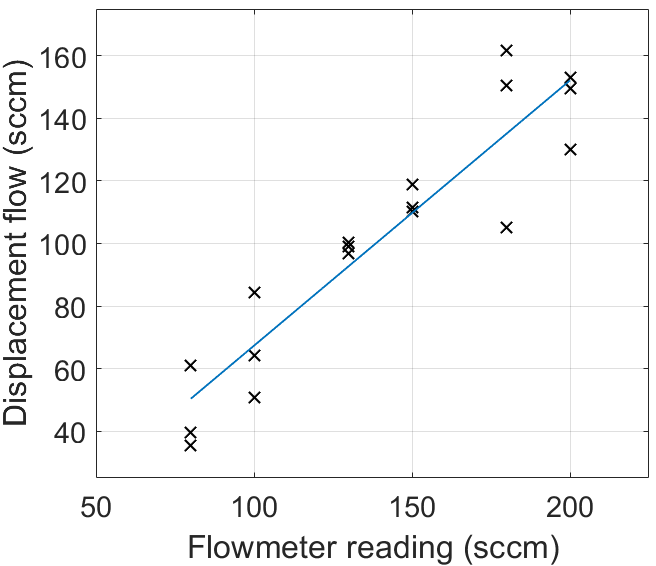
\includegraphics[width=0.5\textwidth,height=\textheight]{figures/ch5/PID_flowmeter.png}

}

\caption{\label{fig-flowmeter-calibration}Calibration curve for the PID
flowmeter, comparing flowmeter readings with flow rate of water
displacement.}

\end{figure}

The time taken to displace a fixed water volume was also measured three
times for a series of constant flow rates through the flowmeter from the
chamber to exhaust. A linear relationship was obtained between flowmeter
readings and actual displacement, as shown in
Figure~\ref{fig-flowmeter-calibration}. Expressing the relationship as
\(D = b_1f + b_2\), where \(f\) is the flowmeter reading and \(D\) is
measured displacement flow, values of \(b_1 = 1.0\pm0.2\) and
\(b_2 = 80\pm25\) were obtained. A 200 sccm flow rate through the
dilution line from the Tylan MFC, corresponding to a \(\sim\) 230 sccm
actual flow rate through the chamber, would therefore be measured as a
\(\sim\) 150 sccm flow rate by the flowmeter. Subsequent measurements
showed that the linear relationship in
Figure~\ref{fig-flowmeter-calibration} breaks down for flowmeter
readings \(\lesssim 75\). For example, a 50 sccm flow on the flowmeter
was found to correspond to 85 sccm of measured displacement flow. By
disconnecting the flowmeter from the PID micropump and closing all
valves out of the manifold except the valve exiting to the flowmeter
(see Figure~\ref{fig-stage-2-pid}), the nominal flow on the MFC could be
directly compared to the flowmeter reading. In this manner, the actual
flow rate of readings \(\lesssim 75\) sccm on the flowmeter could be
quickly obtained.

\hypertarget{sensor-responses-to-vapour-flow}{%
\subsection{Sensor Responses to Vapour
Flow}\label{sensor-responses-to-vapour-flow}}

\begin{figure}

{\centering 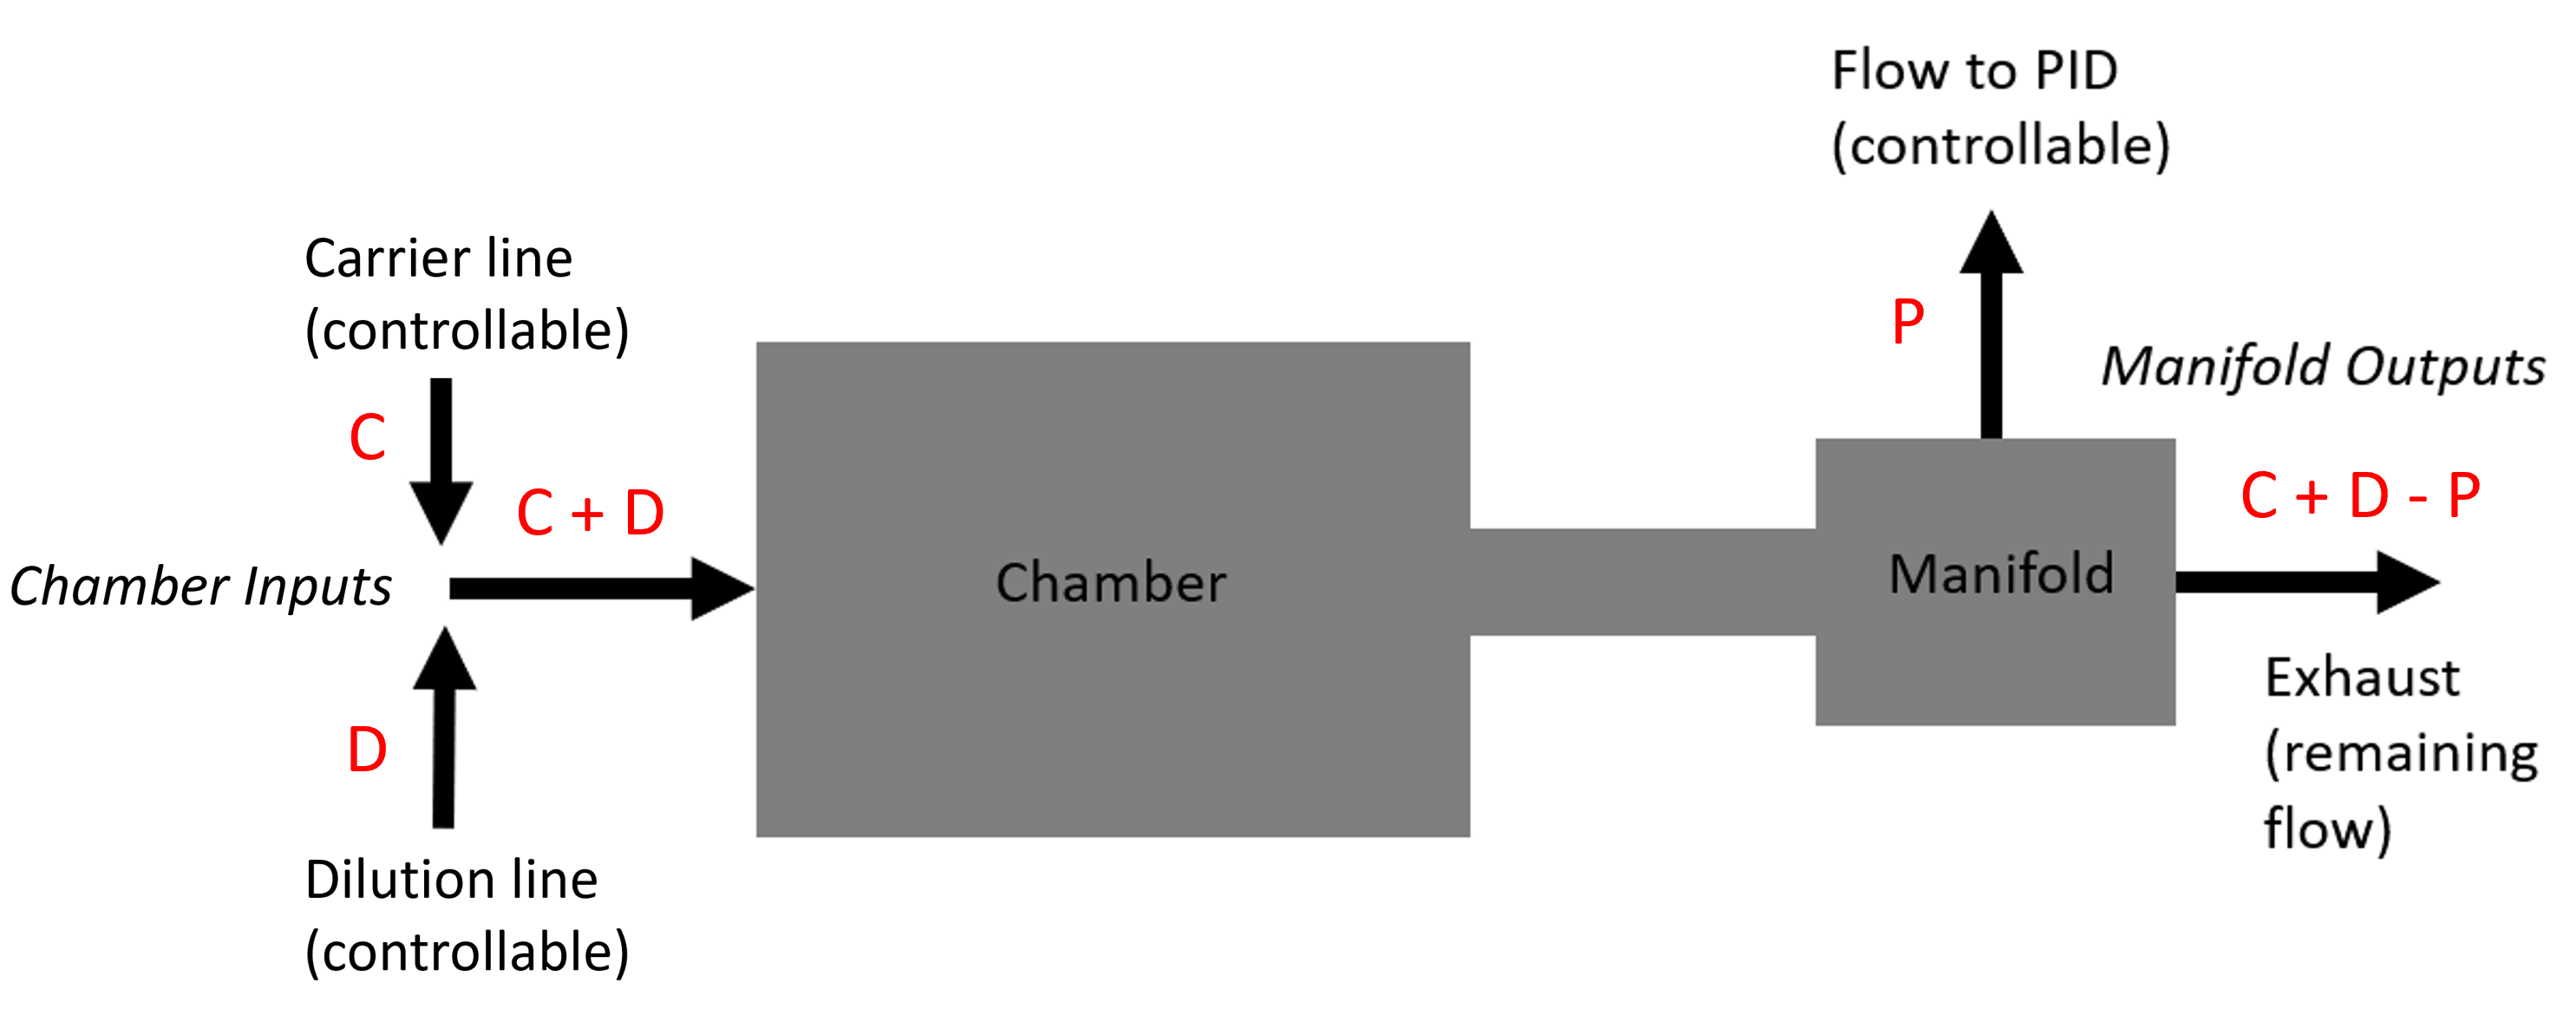
\includegraphics[width=1\textwidth,height=\textheight]{figures/ch5/chamber-manifold-v2.png}

}

\caption{\label{fig-chamber-schematic}Simplified schematic showing the
flow into and out of the device chamber and manifold of the delivery
system. The input flows from the carrier and dilution line are
represented by C and D, and the output flow through the PID is
represented by P. The exhaust can either flow past the relative humidity
indicator or straight to the fumehood. This diagram assumes that flow
through leaks in the chamber and manifold is low enough to be considered
negligible, which was confirmed by leak testing with bubble solution.}

\end{figure}

Once the rate of flow through the device chamber had been calibrated,
the next step was to verify the correct operation of the reference
sensors used in the system. Various flow rates in and out of the chamber
were used to calibrate and verify the reference sensors. These flows in
and out of the chamber are labelled on the simplified schematic in
Figure~\ref{fig-chamber-schematic}.

\hypertarget{relative-humidity-indicator}{%
\subsubsection*{Relative Humidity
Indicator}\label{relative-humidity-indicator}}
\addcontentsline{toc}{subsubsection}{Relative Humidity Indicator}

\begin{figure}

{\centering 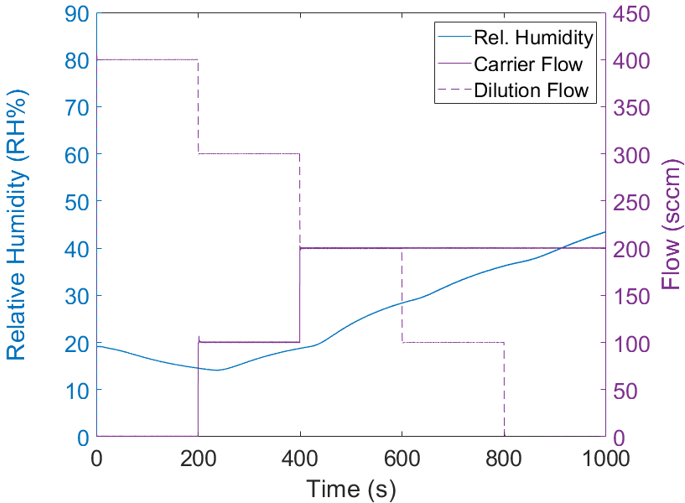
\includegraphics[width=0.7\textwidth,height=\textheight]{figures/ch5/RHI_verification.png}

}

\caption{\label{fig-RHI-verification}Relative humidity readouts from the
relative humidity indicator juxtaposed with flow rates from the dilution
line and carrier lines of the vapour system, with 10 mL deionised water
in the carrier line analyte bottle.}

\end{figure}

To test the relative humidity indicator (RHI), all valves out of the
chamber were sealed except for the valve for the relative humidity
indicator chamber. This meant all flow coming out of the system would
pass through the relative humidity indicator chamber (P = 0 sccm and
exhaust goes to RHI in Figure~\ref{fig-chamber-schematic}). Continuous
nitrogen flow was then placed through the chamber until relative
humidity dropped to about 20\%. 10 mL of deionised water was placed into
the analyte bottle. A series of different flow rates through each line
was sent to the chamber, with the sequence of flow rates shown in
Table~\ref{tbl-RHI-flow-sequence} (t = time, C = carrier line flow rate,
D = dilution line flow rate). Note that between 230 s and 630 s, the
total flow rate remains the same, but the ratio of dilution to carrier
flow differs.

\hypertarget{tbl-RHI-flow-sequence}{}
\begin{longtable}[]{@{}lll@{}}
\caption{\label{tbl-RHI-flow-sequence}Flow sequence for testing relative
humidity indicator.}\tabularnewline
\toprule\noalign{}
t (s) & C (sccm) & D (sccm) \\
\midrule\noalign{}
\endfirsthead
\toprule\noalign{}
t (s) & C (sccm) & D (sccm) \\
\midrule\noalign{}
\endhead
\bottomrule\noalign{}
\endlastfoot
200 & 0 & 400 \\
200 & 100 & 300 \\
200 & 200 & 200 \\
200 & 200 & 100 \\
200 & 200 & 0 \\
\end{longtable}

Figure~\ref{fig-RHI-verification} shows flow purely from the dilution
line decreases humidity as measured by the Telaire sensor, while flow
from the analyte bottle containing deionised water increases humidity,
as expected. It also shows that in regular 200 s intervals, an uptick in
the increase of relative humidity occurs, which then begins to flatten
out. Each gradient uptick occurs about 50 s after a corresponding
increase in flow through the carrier line. It therefore appears that
each interval corresponds to an increase of water vapour flow, where 50
s is the time taken for the increased concentration of water vapour to
first reach the relative humidity indicator.

Over the full 800 s of carrier line flow, relative humidity increases
from a minimum of \(14.0\pm2.0\)\% to a maximum of \(43.6\pm2.0\)\%. The
temperature in the chamber remained between \(21.0\pm0.5\) \(^\circ\)C
and \(22.0\pm0.5\) \(^\circ\)C over the entire measurement period.
Combining equations Equation~\ref{eq-absolute-humidity} and
Equation~\ref{eq-water-vapour-pressure} from
Section~\ref{sec-reference-sensors}, we find that the absolute humidity
in the chamber reaches a low of \(2.6\pm0.4\) gm\(^{-3}\) at 238.1 s,
38.1 s after the initial onset of carrier flow, and a high of
\(8.4\pm0.5\) gm\(^{-3}\) at 998.8 s, after 798.8 s of carrier flow
through the chamber. The clear response of the Telaire RHI to water
vapour flow through the carrier line confirms that this sensor is
working as expected.

\hypertarget{photoionisation-detector-1}{%
\subsubsection*{Photoionisation
Detector}\label{photoionisation-detector-1}}
\addcontentsline{toc}{subsubsection}{Photoionisation Detector}

\begin{figure}

\begin{minipage}[t]{0.20\linewidth}

{\centering 

~

}

\end{minipage}%
%
\begin{minipage}[t]{0.60\linewidth}

{\centering 

\raisebox{-\height}{

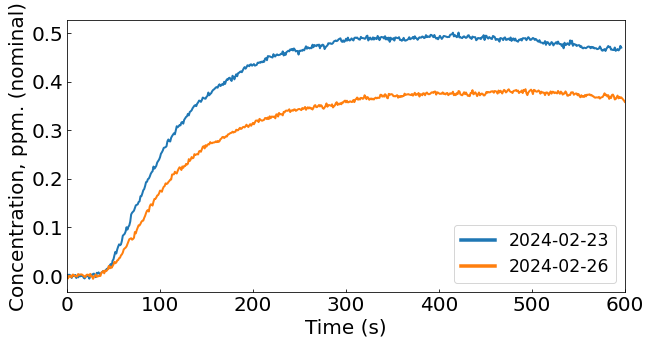
\includegraphics{figures/ch5/240223_240226_comparison_unnormalised.png}

}

}

\subcaption{\label{fig-ethex-comparison-unnormalised}}
\end{minipage}%
%
\begin{minipage}[t]{0.20\linewidth}

{\centering 

~

}

\end{minipage}%
\newline
\begin{minipage}[t]{0.20\linewidth}

{\centering 

~

}

\end{minipage}%
%
\begin{minipage}[t]{0.60\linewidth}

{\centering 

\raisebox{-\height}{

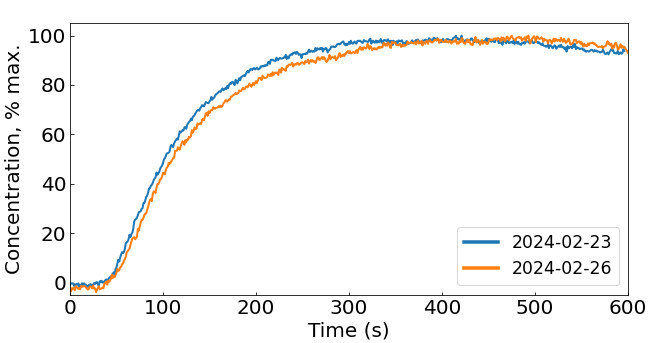
\includegraphics{figures/ch5/240223_240226_comparison.png}

}

}

\subcaption{\label{fig-ethex-comparison}}
\end{minipage}%
%
\begin{minipage}[t]{0.20\linewidth}

{\centering 

~

}

\end{minipage}%

\caption{\label{fig-PID-EtHex-response}The response of the
photoionisation detector to ethyl hexanoate vapour over 600 s of
exposure is shown relative to the 200 sccm nitrogen flow baseline in
(a), and normalised with respect to the maximum reading in (b).}

\end{figure}

To test the photoionisation detector, the device chamber and carrier
line were first purged of vapour through the exhaust using a roughing
pump, with the PID valve closed to protect it from the pump. The PID
valve was then opened, the micropump was set to 150 sccm as read by the
flowmeter. During testing with the PID, the total flow into the chamber
was set at 200 sccm as read by the mass flow controllers. The
calibration curves in Section~\ref{sec-flow-calibration} show that the
actual flow C + D was then therefore approximately the same as the
actual flow rate into the PID, P. A flow of 200 sccm nitrogen was placed
through the dilution line to the chamber for 10 minutes until successive
concentration readings from the PID were either approximately constant,
or until baseline drift was small enough to be considered negligible.
These measurements were then used as the baseline (0 ppm) for subsequent
measurements. 5 mL of the volatile organic compound ethyl hexanoate
(EtHex) was placed into the analyte bottle. A flow of 150 sccm was then
sent through the carrier line and 50 sccm through the dilution line for
600 s. The same procedure was performed on two separate days spaced
three days apart to check that the measured PID response to ethyl
hexanoate vapour pumped out of the manifold was repeatable.

The responses from each day are shown in
Figure~\ref{fig-PID-EtHex-response}. In
Figure~\ref{fig-ethex-comparison-unnormalised}, the response from each
day is shown unnormalised, with the parts per million concentration
shown relative to the nitrogen baseline as recorded.

\hypertarget{summary}{%
\section{Summary}\label{summary}}

\cleardoublepage
\phantomsection
\addcontentsline{toc}{part}{Appendices}
\appendix

\hypertarget{sec-vapour-sensor-components}{%
\chapter{Vapour System Hardware}\label{sec-vapour-sensor-components}}

\hypertarget{tbl-vapour-sensor-components}{}
\begin{longtable}[t]{>{\raggedright\arraybackslash}p{5.5cm}>{\raggedright\arraybackslash}p{4.5cm}>{\raggedright\arraybackslash}p{3.75cm}}
\caption{\label{tbl-vapour-sensor-components}Major components used in construction of the vapour delivery system
described in this thesis. }\tabularnewline

\toprule
Description & Part No. & Manufacturer\\
\midrule
Mass flow controller, 20 sccm full scale & GE50A013201SBV020 & MKS Instruments\\
Mass flow controller, 200 sccm full scale & GE50A013202SBV020 & MKS Instruments\\
Mass flow controller, 500 sccm full scale & FC-2901V & Tylan\\
Analogue flowmeter, 240 sccm max. flow & 116261-30 & Dwyer\\
Micro diaphragm pump & P200-B3C5V-35000 & Xavitech\\
\addlinespace
Analogue flow controller, for micro diaphragm pump & X3000450 & Xavitech\\
10 mL Schott bottle & 218010802 & Duran\\
PTFE connection cap system & Z742273 & Duran\\
Baseline VOC-TRAQ flow cell, red & 043-951 & Mocon\\
Humidity and temperature sensor & T9602 & Telaire\\
\addlinespace
Enclosure, for humidity and temperature sensor & MC001189 & Multicomp Pro\\
\bottomrule
\end{longtable}

\hypertarget{sec-python}{%
\chapter{Python Code for Data Analysis}\label{sec-python}}

\hypertarget{code-repository}{%
\section{Code Repository}\label{code-repository}}

The code used for general analysis of field-effect transistor devices in
this thesis was written with Python 3.8.8. Contributors to the code used
include Erica Cassie, Erica Happe, Marissa Dierkes and Leo Browning. The
code is located on GitHub and the research group OneDrive, and is
available on request.

\hypertarget{sec-histogram-analysis}{%
\section{Atomic Force Microscope Histogram
Analysis}\label{sec-histogram-analysis}}

The purpose of this code is to analyse atomic force microscope (AFM)
images of carbon nanotube networks in .xyz format taken using an atomic
force microscope and processed in Gwyddion (see
\textbf{?@sec-afm-characterisation}). It was originally designed by
Erica Happe in Matlab, and adapted by Marissa Dierkes and myself for use
in Python. The code imports the .xyz data and sorts it into bins 0.15 nm
in size for processing. To perform skew-normal distribution fits, both
\emph{scipy.optimize.curve\_fit} and \emph{scipy.stats.skewnorm} modules
are used in this code.

\hypertarget{sec-raman-analysis}{%
\section{Raman Spectroscopy Analysis}\label{sec-raman-analysis}}

The purpose of this code is to analyse a series of Raman spectra taken
at different points on a single film (see
\textbf{?@sec-raman-characterisation}). Data is imported in a series of
tab-delimited text files, with the low wavenumber spectrum (100
cm\(^{-1} - 650\) cm\(^{-1}\)) and high wavenumber spectrum (1300
cm\(^{-1} - 1650\) cm\(^{-1}\)) imported in separate datafiles for each
scan location.

\hypertarget{sec-field-effect-transistor-analysis}{%
\section{Field-Effect Transistor
Analysis}\label{sec-field-effect-transistor-analysis}}

The purpose of this code is to analyse electrical measurements taken of
field-effect transistor (FET) devices. Electrical measurements were
either taken from the Keysight 4156C Semiconductor Parameter Analyser,
National Instruments NI-PXIe or Keysight B1500A Semiconductor Device
Analyser as discussed in \textbf{?@sec-electrical-characterisation}; the
code is able to analyse data in .csv format taken from all three
measurement setups. The main Python file in the code base consists of
three related but independent modules: the first analyses and plots
sensing data from the FET devices, the second analyses and plots
transfer characteristics from channels across a device, and the third
compares individual channel characteristics before and after a
modification or after each of several modifications. The code base also
features a separate config file and style sheet which govern the
behaviour of the main code. The code base was designed collaboratively
by myself and Erica Cassie over GitHub using the Sourcetree Git GUI.


\backmatter
\printbibliography


\end{document}
